%%%%%%%%%%%%%%%%%%%%%%%%%%%%%%%%%%%%%%%%%%%%%%%%%%%%%%%%%%%%%%%%%%%%%%%%
%    INSTITUTE OF PHYSICS PUBLISHING                                   %
%                                                                      %
%   `Preparing an article for publication in an Institute of Physics   %
%    Publishing journal using LaTeX'                                   %
%                                                                      %
%    LaTeX source code `ioplau2e.tex' used to generate `author         %
%    guidelines', the documentation explaining and demonstrating use   %
%    of the Institute of Physics Publishing LaTeX preprint files       %
%    `iopart.cls, iopart12.clo and iopart10.clo'.                      %
%                                                                      %
%    `ioplau2e.tex' itself uses LaTeX with `iopart.cls'                %
%                                                                      %
%%%%%%%%%%%%%%%%%%%%%%%%%%%%%%%%%%
%
%
% First we have a character check
%
% ! exclamation mark    " double quote  
% # hash                ` opening quote (grave)
% & ampersand           ' closing quote (acute)
% $ dollar              % percent       
% ( open parenthesis    ) close paren.  
% - hyphen              = equals sign
% | vertical bar        ~ tilde         
% @ at sign             _ underscore
% { open curly brace    } close curly   
% [ open square         ] close square bracket
% + plus sign           ; semi-colon    
% * asterisk            : colon
% < open angle bracket  > close angle   
% , comma               . full stop
% ? question mark       / forward slash 
% \ backslash           ^ circumflex
%
% ABCDEFGHIJKLMNOPQRSTUVWXYZ 
% abcdefghijklmnopqrstuvwxyz 
% 1234567890
%
%%%%%%%%%%%%%%%%%%%%%%%%%%%%%%%%%%%%%%%%%%%%%%%%%%%%%%%%%%%%%%%%%%%
%
\documentclass[12pt]{iopart}
%Uncomment next line if AMS fonts required
%\usepackage{iopams}  
\usepackage{hyperref,tikz,array}
\usepackage[export]{adjustbox}
\usepackage{gensymb,eurosym}
\usepackage[numbers]{natbib}
\usepackage[inline]{enumitem}
\usepackage[all]{hypcap}
\pdfminorversion=4
\graphicspath{{Images/}}
\newcolumntype{P}{>{\raggedright\arraybackslash}p}
\usetikzlibrary{arrows.meta, shapes.geometric}
\newcommand{\rpm}{\raisebox{.3ex}{$\scriptstyle\pm$}}
\hypersetup{hidelinks}

\begin{document}
\title[Reusing wastewater in agriculture: a WEF Nexus assessment in the NWSAS]{Reusing wastewater for agricultural irrigation: a water-energy-food Nexus assessment in the North Western Sahara Aquifer System}

\author{C. Ramirez $^{1}$, Y. Almulla $^{1}$ and F. Fuso-Nerini $^{1}$}

\address{$^{1}$ KTH Royal Institute of Technology, Stockholm, Sweden}
\ead{camilorg@kth.se}
\vspace{10pt}
\begin{indented}
\item[]\today
\end{indented}

\begin{abstract}
The North Western Sahara Aquifer System stands out as one of the water scarcest regions worldwide. In recent decades agriculture activity has grown exerting pressure on groundwater resources and pumping energy requirements. In this study, a nexus approach was used to assess the effect of capturing, treating and reusing wastewater for irrigation. GIS-based tools were used to capture the systems spatial dimension, enabling to match wastewater supply and water demand points, identify demand hotspots and evaluate techno-economically viable wastewater treatment options. Eight  wastewater treatment technologies were evaluated, making use of a Levelised Cost of Water methodology to identify the least-cost system. Six scenarios were constructed based on population water requirements and water-consumption behaviour of farmers towards changes in irrigation water pricing. The identified least-cost technologies, showed clear trade-offs related to treatment capacity. The reuse of treated wastewater in agricultural irrigation, showed improvement of groundwater stress, reducing up to 38\% water abstractions and lowering stress levels from medium-to-high to low-to-medium. Furthermore, reuse of wastewater decreased dependency on groundwater pumping and the overall energy-for-water requirements. However, to effectively preserve water resource, measures as better water pricing mechanisms, management strategies to improve water productivity and adoption of more efficient irrigation schemes are needed.
\end{abstract}

% Uncomment for keywords
\vspace{1pc}
\noindent{\it Keywords}: water, energy, agriculture, Nexus, wastewater reuse, NWSAS, GIS.

% Uncomment for Submitted to journal title message
\submitto{\ERL}
%
% Uncomment if a separate title page is required
%\maketitle
% 
% For two-column output uncomment the next line and choose [10pt] rather than [12pt] in the \documentclass declaration
% \ioptwocol
%
\section{Introduction}
% Add selected references from 2 fonts: other nexus assessments looking at wastewater, other assessments and literature on NWSAS. The idea here is that you show that there are some clear gaps in literature, that get you to your research questions, that you answer in the paper. As starting point the next text can help for the studies taken in the NWSAS. It will need some edition as some parts were used for the previous paper. Also, should I cite our work on the NWSAS too? moreover, it is necessary to explain the transboundary characteristic of the basin and why is it key for the region.

% Start with introduction on water scarcity issue and literature on wastewater as a resource, covering its current state and reuse potential. Link this literature to the nexus-SDGs nature publications, highlighting the key connections of the water SDG to the health and sanitation SDG (for which wastewater treatment is key) and the direct link to energy and food (due to water availability for irrigation). In here mention some wastewater-energy nexus perspective worldwide. Then, look into the assessments and literature in the region and the wastewater treatment and reuse studies (Mediterranean and NWSAS). Finally, look into the wef nexus studies of the region (MENA and NWSAS) and explain gaps with nexus on wastewater-energy-food perspective both globally and in the region, and highlight the main objective of the research.

It is well known that variations on the dynamics of the water cycle are causing disparity in water demand and supply globally \cite{FAO2015,unescoWastewaterUntappedResource2017}. This, has led to recurrent and prolonged drought periods pushing two-thirds of the worlds population to experience water scarcity for at least one month a year \cite{Mekonnene1500323}. Such problematic makes utterly challenging to cope with an expected increase in water demand due to agricultural, industrial and population growth over the next decades \cite{IFPRI2017}. Moreover, inefficient use of water aggravates the problem and puts more pressure into the system. Worldwide, agriculture irrigation consumes around 70\% of all bluewater resources, of which 45\% are not used and returned as untreated drainage \cite{unescoWastewaterUntappedResource2017}. In addition, around 70\% of bluewater abstractions for population uses are returned as wastewater \cite{unescoWastewaterUntappedResource2017}. Overall, 56\% of all bluewater abstractions are wasted, however, this resource still carries a vast potential. Nutrients can be recovered from wastewater and subsequently used as high-quality fertilizers for food production \cite{moEnergyNutrientsWater2013a}. Heat and electricity can be generated by using extracted biogas from anaerobic digestion processes, biosolids incineration, effluents hydropower, heat pumps and bioelectrochemical systems, among others \cite{moEnergyNutrientsWater2013a}. Whereas, high quality treated wastewater can be reused for agricultural irrigation, ecosystems services maintenance, industrial processes and groundwater replenishment \cite{moEnergyNutrientsWater2013a}.

Wastewater treatment and reuse has been internationally recognized as one of the best measures to ease water scarcity as it can substantially increase water availability \cite{unescoWastewaterUntappedResource2017,GARCIA2015154}. According to the AQUASTAT database, the amount of industrial and municipal wastewater treated worldwide, ranges from 8\% to 70\% in low-income and high-income countries respectively. However, agricultural drainage water is almost never collected or treated, and only a marginal amount of the treated wastewater is actually reused \cite{unescoWastewaterUntappedResource2017}. Non-treated wastewater that runs freely to the environment, often poses severe environmental and health consequences, polluting groundwater aquifers, rivers, lakes, soils and food, among others. Nonetheless, there are several cases of success where treated wastewater reuse has substantially improved agricultural irrigation (aiding food production), incremented water availability for ecosystem services and supported aquifer recharge \cite{hettiarachchiSAFEUSEWASTEWATERa, halalshehPolicyGovernanceFramework2018, mahjoubPublicAcceptanceWastewater2018, zuurbierUseWastewaterManaged2018, hussainSustainableUseManagement2019}.

Wastewater reuse plays an important role for sustainable development as it is essential for achieving SDG 6 on clean water and sanitation. Key targets of SDG 6 are to improve water quality by reducing by half the amount of non-treated wastewater and increasing recycling and safe reuse globally \cite{UNSDGs2019, tortajadaContributionsRecycledWastewater2020}. The achievement of such targets can substantially increase availability of clean water resources for all uses, not available otherwise. This also means that discharge of cleaner wastewater in ecosystems can support SDG 14 on life below water and SDG 15 on life on land \cite{UNSDGs2019, tortajadaContributionsRecycledWastewater2020}. Furthermore, synergies and trade-offs with virtually all SDGs exist \cite{WaterSanitationInterlinkages2016}. The strong interconnection between SDGs \cite{WaterSanitationInterlinkages2016,fusoneriniMappingSynergiesTradeoffs2018,fusoneriniConnectingClimateAction2019}, supports the use of holistic approaches to evaluate actions towards achieving sustainable development targets, commonly known as Nexus approaches \cite{liuNexusApproachesGlobal2018,bleischwitzResourceNexusPerspectives2018,olawuyiSustainableDevelopmentWaterenergyfood2020,simpsonDevelopmentWaterEnergyFoodNexus2019,hoffNexusApproachMENA2019}. Links between wastewater reuse and SDG 2 on zero hunger (mainly due to sustainable food production and resilient agricultural practices), SDG 7 on affordable and clean energy (mainly due to improved energy efficiency and increasing the share of renewable energy) and SDG 13 on climate action (mainly due to strengthen resilience and adaptive capacity to climate-related hazards), can be noticed as a clear water, energy, food and climate Nexus \cite{WaterSanitationInterlinkages2016,liuNexusApproachesGlobal2018,hoffNexusApproachMENA2019}.

Nexus approaches have been widely used for evaluating interlinkages between resource systems, trying to identify challenges, synergies, trade-offs and evaluate holistic solutions, specially in the MENA region \cite{hoffNexusApproachMENA2019,kingRapidAssessmentWater2015}. Furthermore, Nexus thinking is also gaining attention in transboundary resources settings \cite{uneceReconcilingResourceUses2015,kingRapidAssessmentWater2015}. Such is the case of the North Western Sahara Aquifer System (NWSAS). The NWSAS is located in North Africa covering large parts of Algeria, Tunisia and Libya, and it holds invaluable groundwater resources to maintain livelihood in the region \cite{BetterValorizationIrrigation2015}.

The main scientific studies on the NWSAS have been conducted in the form of joint efforts between Algeria, Tunisia, and Libya \cite{abuzeidNorthWesternSahara2015}. Such efforts have identified challenges and risks that the NWSAS has been facing mainly in terms of water scarcity and utilization \cite{BetterValorizationIrrigation2015}. Research outcomes have achieved common databases containing over 9,000 water points, developed hydraulic models to assess impacts of water withdrawals, set consultation mechanisms for joint management of water resources, evaluated new water withdrawal potential and the associated risk of future exploitation, identified the inefficiency of irrigation, the inadequate valorization of water and the degradation of soil quality in the region \cite{khaterNorthWesternSahara2014,abuzeidNorthWesternSahara2015,BetterValorizationIrrigation2015,Socioeconomicaspectsirrigation2014}. Moreover, technical innovation pilots have been implemented in the NWSAS under four themes \cite{ossAgriculturalDemostrationPilots2014}: 1) solar energy for pumping water, both for irrigation and for drainage evacuation, 2) brackish water valuation through demineralization, 3) rehabilitation of lands degraded due to water stagnation, and 3) irrigation efficiency and agricultural intensification. 

Although, the joint efforts of the three countries and the OSS have been substantial and key for understanding the complexity and vulnerability of the NWSAS system, the components of the research have been heavily driven by understanding water issues---with a lesser focus on the sectors that drive or are needed to support the supply of water. In addition, the wastewater reclaim treatment and reuse potential has not yet been explored at the basin level, neither the synergies and trade-offs it may have with the energy, water and agricultural sectors. In general, wastewater treatment and reuse measures have been commonly evaluated with a water centred approach, often overlooking energy requirements and its implications. On the other hand, water-energy nexus approaches exploring the wastewater topic, have usually focused on the energy and nutrients recovery potential from wastewater. Moreover, feasibility studies of reusing wastewater, have assessed potential on specific sites (e.g. wastewater treatment plants) or at the national level based on general statistics. To date, a gap was found into how to determine the potential for wastewater treatment, reclaim and reuse, taking into account potential treatment technologies, energy demand implications and effects on the water system. In this paper, a Nexus approach is used to asses the impact that reclaiming, treating and reusing wastewater (i.e. in agricultural irrigation), may have in the water, food and energy systems in the NWSAS, making use of Geographic Information Systems (GIS) and a Levelised Cost of Water (LCOW) methodology.

% In 1999 a multi-phase project led by the Sahara and Sahel Observatory (OSS), launched with the purpose of ensuring control over potential impacts of transboundary water resources (Khater, 2014). The first phase of the program ended in year 2002, achieving a common database containing over 9,000 water points, a hydraulic model to assess impacts of water withdrawals, and a consultation mechanism for joint management of water resources that evolved to a permanent structure in 2008 (AbuZeid and Elrawady, 2015; Khater, 2014). The modelling efforts undertaken in the first phase of the project were aimed at identifying new water withdrawal potential in the aquifer and the associated risk of future exploitation, projecting scenarios to year 2050 (Khater, 2014). Moreover, from year 2003, new studies were carried out as part of the second phase of the project, in order to make a diagnosis of the agriculture sector, in reference to the hydraulic aspects of the basin (OSS, 2015). The study helped to identify the inefficiency of irrigation, the inadequate valorization of water and the degradation of soil quality in the NWSAS.

% In 2009, OSS continued with the third phase of the project developing a study on water valorization in the NWSAS, focused on enhancing sustainable development in the region (OSS, 2015). The study consisted of two main components: a socio-economic component that analyzes the modes of operation of agricultural systems and understanding the behaviour of the irrigators (OSS, 2014b). For this, several surveys were conducted to almost 3,000 farmers. The second component is known as “demonstration pilots”, consisted on implementing technical innovations aimed at testing their feasibility and acceptance on the farmers level, with the purpose of saving and valorizing water in the NWSAS basin (OSS, 2014c). These pilots were comprised of six projects that focused on certain areas (oases) and can be catalogued into four themes: 1) solar energy for pumping water, both for irrigation and for drainage evacuation, 2) brackish water valuation through demineralization, 3) rehabilitation of lands degraded due to water stagnation, and 3) irrigation efficiency and agricultural intensification.

% Although the joint efforts of the three countries and the OSS have been substantial and key for understanding the complexity and vulnerability of the NWSAS system, the components of the research have been heavily driven by understanding water issues---with a lesser focus on the sectors that drive or are needed to support the supply of that water. Another limitation is that most of the pilot studies covered certain areas on the NWSAS and no study really considered the entire NWSAS especially when it comes to energy and water aspects. In this regard, an evaluation of the resources in a nexus context has not yet been performed. A regional study that tackles interlinkages between the agriculture, water and energy sectors in the NWSAS, is necessary to achieve a joint planning and sustainable development of the three sectors in the basin and all the implicated countries. 
% \cite{gremillionWastewaterResourceWaterWasteEnergy}

\section{Methodology}
The methods used in this study follow those of the framework presented in \cite{ramirezgomezTechnoeconomicGISbasedModel2018}, with some key additions and improvements. The summary of the methodology and methods is presented in \fref{fig:framework}.

\begin{figure*}[!h]
	\centering
	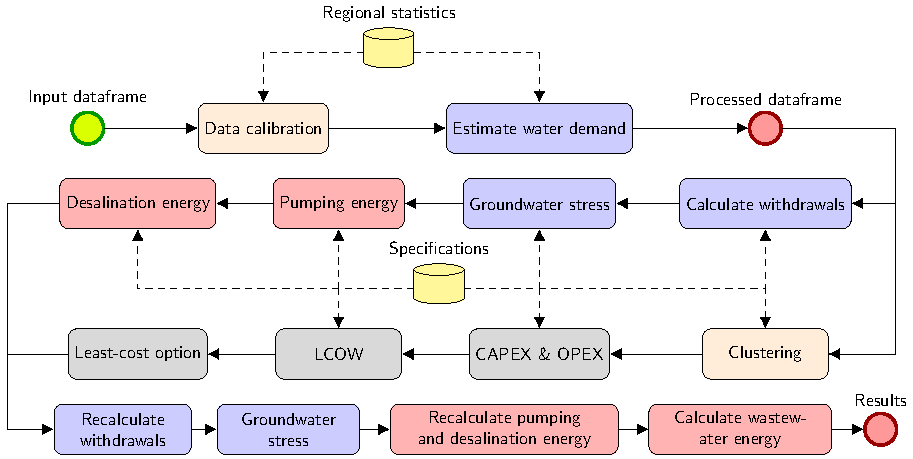
\includegraphics[width=\textwidth]{Framework}
	\caption{Methodology flow diagram.}
	\label{fig:framework}
\end{figure*}

The water-agriculture-energy system evaluated for the NWSAS consisted of the extraction of groundwater resources, desalination of brackish water when needed, water demand for domestic and agricultural irrigation purposes, reclaim of domestic wastewater and agricultural drainage (i.e. tailwater), treatment of reclaimed wastewater, and treated wastewater reuse in agricultural irrigation. A schematic of the system is presented in \fref{fig:system_reuse}.

\begin{figure*}[!h]
	\centering
	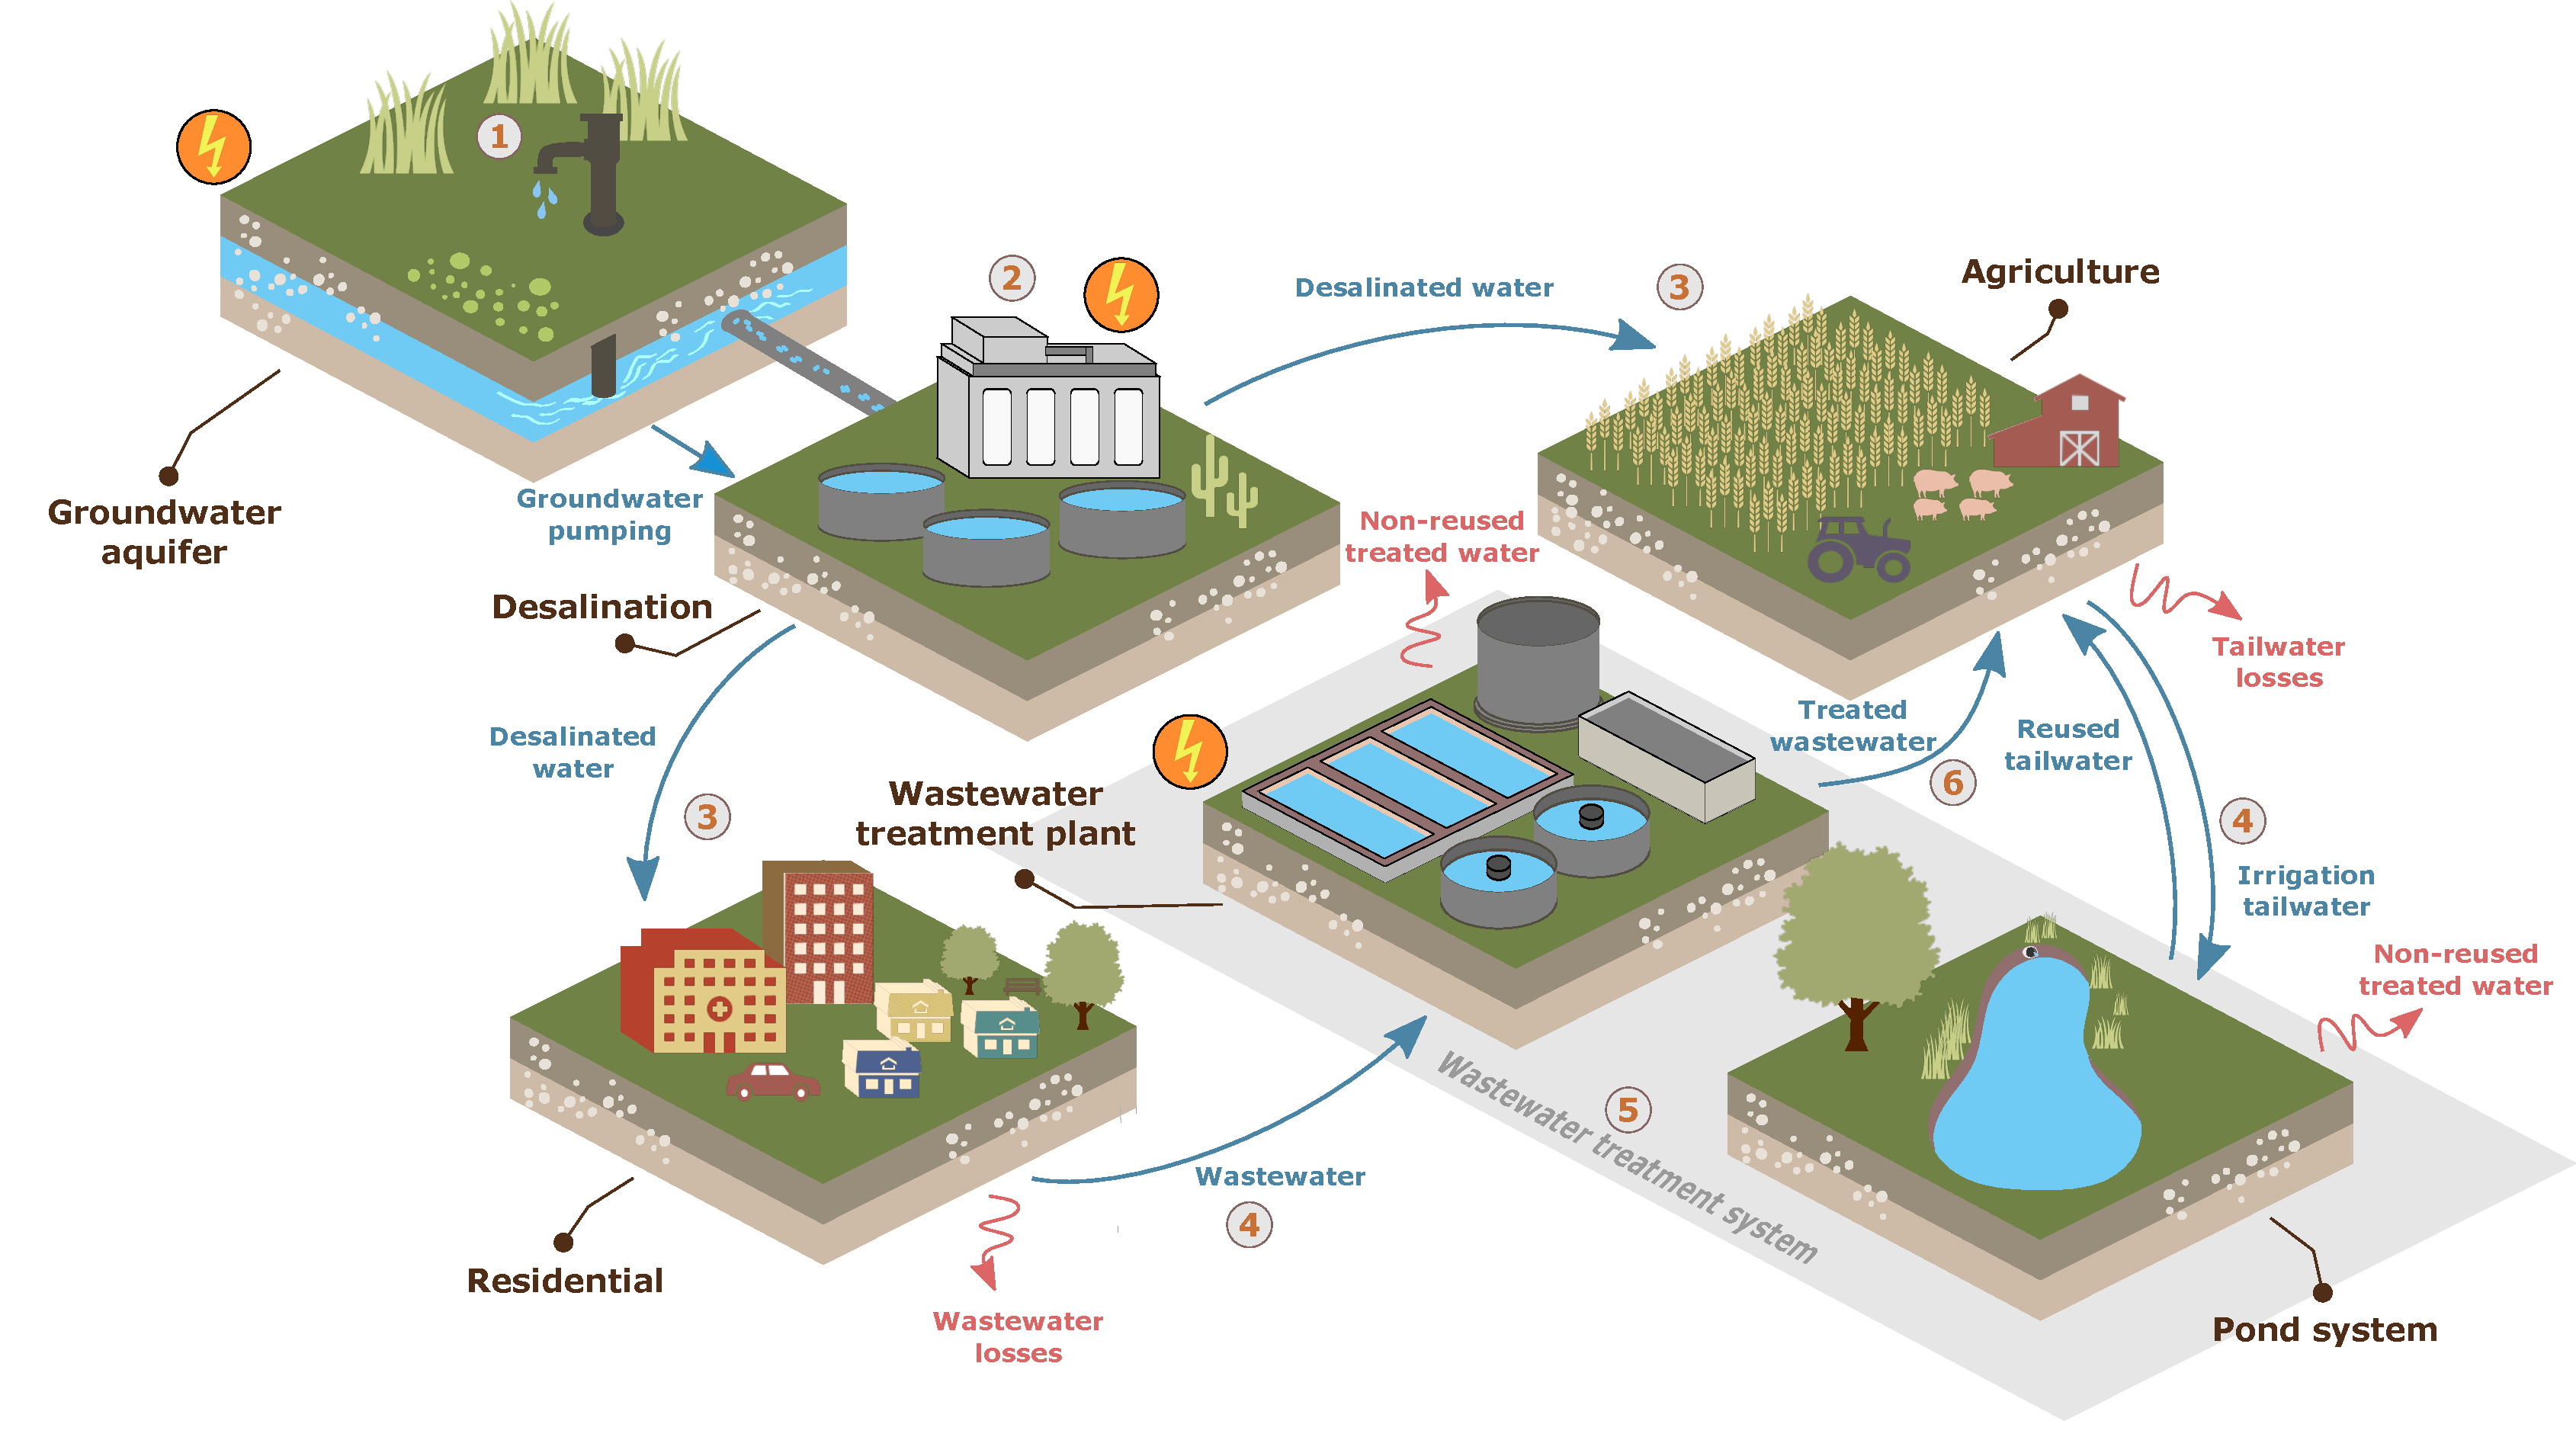
\includegraphics[width=\textwidth]{System_reuse}
	\caption{NWSAS components and resource streamflows - WWR scenarios.}
	\label{fig:system_reuse}
\end{figure*}

All water requirements for population consumption and agricultural irrigation were assumed to be supplied by the groundwater aquifer and that such water is desalinated whenever the TDS levels are above 1,000 mg/l \cite{fao1985water}. Afterwards, the water is allocated for population consumption and agricultural irrigation. 
% Finally, wastewater from population and tailwater from agriculture is disposed to the environment without any adequate treatment. 
The recharge rate $R$ for the entire aquifer was taken as 1.1 billion cubic meters of water per year, which for the area of the aquifer, is an equivalent water column of 1.06 mm per year \cite{BetterValorizationIrrigation2015}. Furthermore, no environmental flow was considered.

Six wastewater treatment and reuse scenarios were analysed, evaluating three irrigation water pricing regimes and two levels of population water consumption. Irrigation water pricing regimes were taken from \cite{Socioeconomicaspectsirrigation2014}, were it was found that the irrigation water demand per hectare throughout the NWSAS basin is heavily dependent on the supply water cost. Three different regimes for water users exist: 

\begin{enumerate}
	\item \textbf{Private water users:} private farmers that pay the full price of water without any subsidy. The average level of water demand is around 10,512 m\textsuperscript{3}/ha. The \citet{Socioeconomicaspectsirrigation2014} found, that farmers belonging to this regime, have higher water productivity. 
% 	This means that, they have a better use of the resource, obtaining more product while using less amount of irrigation water per hectare.
	\item \textbf{Subsidized water users:} users that have access to water subsidized to some extent. The average water demand is 15,334 m\textsuperscript{3}/ha.
	\item \textbf{Free water users:} farmers that have free access to water, meaning that the government fully subsidize the price of water and that the resource can be utilized without limitations. The average irrigation water demand is 21,215 m\textsuperscript{3}/ha.
\end{enumerate}

Water demand in the subsidized and free regimes, constitutes a 45.8\% and a 101.8\% increase in irrigation water requirements compared to the private regime respectively. This suggests a strong price elasticity of the irrigation water demand and/or the use of lower efficiency irrigation technologies \cite{Socioeconomicaspectsirrigation2014}.

On the other hand, two levels of population water consumption were analysed based on the work of \citet{Householdwaterconsumption2014}:

\begin{enumerate}
    \item \textbf{Low level:} an average water consumption per capita of 55 m\textsuperscript{3}/year.
    \item \textbf{High level:} an average water consumption per capita of 73 m\textsuperscript{3}/year.
\end{enumerate}

In addition, a sensitivity analysis was performed on the groundwater quality and depth to groundwater levels, in order to asses the impact they pose to the energy-for-water requirements (\tref{tbl:sensitivy}). This parameters were selected, as the water security of the aquifer highly depends on the water table levels and the quality of the resource, directly affecting food security as well.

\begin{table}[!ht]
	\caption{\label{tbl:sensitivy}Sensitivity parameters.}
	\begin{indented}
	\item[]\begin{tabular}{@{}l l l l}
		\br
		Parameter & Low & middle & high\\
		\mr
		Groundwater quality & -10 meters & current level & +10 meters\\
		Depth to groundwater & -50\% & current level & +50\%\\
		\br
	\end{tabular}
	\end{indented}
\end{table}

% \noindent Groundwater quality:
% \begin{itemize}
% 	\item Low: -50\% of the current TDS levels,
% 	\item Neutral: the current TDS levels,
% 	\item High: +50\% of the current TDS levels.
% \end{itemize}

% \textbf{Depth to groundwater:}
% \begin{itemize}
% 	\item Low: -10 meters of the current depth to groundwater levels,
% 	\item Neutral: the current depth to groundwater levels,
% 	\item High: +10 meters of the current depth to groundwater levels.
% \end{itemize}

% \subsection{Geographic Information Systems analysis}

% \begin{table*}[b]
% 	\caption{\label{tbl:datasources}Geographic Information System data sources}
%     {\footnotesize
%     \begin{tabular*}{\textwidth}{@{}P{1.4in} P{1in} l P{1.2in} l l@{}}
%     \br
%     Layer & Coverage & Format & Resolution & Year & Source\\
%     \mr
%     Population & Algeria, Tunisia, Libya & raster (tif) & 100 m grid cell & 2015 & \cite{Worldpop2012}\\\ms
%     Depth to groundwater & Africa & txt table & 5 km grid cell & 2012 & \cite{Quantitativemapsgroundwater2012a}\\\ms
%     Administrative boundaries & Africa & shapefile & Individual country polygons & 2017 & \cite{Humanitarian2017}\\\ms
%     Administrative boundaries & Algeria, Tunisia, Libya & shapefile & Level 1 (provinces) polygons & 2015 & \cite{GADM}\\\ms
%     Transboundary aquifers borders & Global & shapefile & Individual polygons & 2015 & \cite{IGRAC}\\\ms
%     Groundwater quality & NWSAS Basin & data points & 206 data points & 2016 & RA*\\\ms
%     Digital Elevation Data* & Africa & raster (tif) & 1, 3 and 15 arc second & 2014 & \cite{DEM2014}\\\ms
%     Land cover & Africa & raster (tif) & 20 m grid cell & 2016 & \cite{ESA2017}\\\ms
%     Aquifer boundaries & NWSAS basin & shapefile & Individual polygons & - & RA*\\\ms
%     Climate data & Global & raster (tif) & 30 arc second, monthly & 1970-2000 & \cite{WorldClimGlobalClimate}\\
%     \br
%     \end{tabular*}\\
%     ~* Regional Authorities.
%     }
% \end{table*}

The most up-to-date open source data available was collected and processed using the open source Geographic Information System software QGIS. A data package comprising the geospatial characteristics of the study area was created, in order to capture key information to make the WEF nexus analysis possible. The relevant layers are identified and described in \tref{tbl:datasources}.

% All data layers were converted into matching units, re-projected into the Sud Algerie Degree projection (ESRI: 102592)---This projection was selected as it produces minimal distortions in the analysis area---, re-scaled to the same resolution and, when only individual data points were available, interpolated to extend the data to the entire analysed area (i.e. for the Groundwater quality layer). Furthermore, all layers were merged into a large data frame.

% \subsection{Data calibration}
% The \textit{population} and the \textit{irrigated area} layers were calibrated to match regional statistics. The calibration was performed using the fraction given between the regional statistical data (i.e. total population or total irrigated area), and the sum of all data points of the layer in question. The statistical data was available as per country basis. Thus, the calibration process was performed for the basin areas within each country, using their specific information (see \tref{tbl:regionalstats}).

% \begin{table*}[!h]
% 	\caption{\label{tbl:regionalstats}NWSAS population and irrigated area statistics for year 2015, subdivided per country area inside the basin. Data source: \cite{BetterValorizationIrrigation2015}}
% 	\begin{indented}
% 	\item[]\begin{tabular}{@{}l*{4}{r}}
% 		\br
% 		Parameter & Total & Algeria & Tunisia & Libya\\
% 		\mr
% 		NWSAS Population & 6,376,367 & 4,240,888 & 617,168 & 1,518,311\\
% 		NWSAS Irrigated area (Ha) & 469,529 & 237,485 & 56,547 & 175,497\\
% 		\br
% 	\end{tabular}
% 	\end{indented}
% \end{table*}

% Moreover, to calibrate the irrigated area data, an algorithm was run to ensure that non of the data cells had more than 100\% of its area covered by irrigated land.
 
% \subsection{Population and irrigation water withdrawals}
% The calculation of total water withdrawals $ww_{tot,i}$ was performed according to \eref{eq:waterwithdrawals}. Population water withdrawals were calculated as the product between the population count in each data cell ($Pop_{i}$) and the specific water demand per capita ($wpc_{i}$) for the region. Similarly, withdrawals from irrigated agriculture were calculated as the product between the irrigated area inside each data cell ($IrrArea_{i}$) and the specific water demand per cultivated hectare ($wpha_{i}$) for the region.

% \begin{equation}\label{eq:waterwithdrawals} 
% ww_{tot,i} = Pop_{i}\cdot wpc_{i} +IrrArea_{i}\cdot wpha_{i} 
% \end{equation}

% For the baseline, a level of water withdrawals per capita $wpc$ of 55 cubic meters per year was assumed with a population growth of 1\% per year \cite{Householdwaterconsumption2014}. Moreover, all cropland area within the aquifer was considered to be irrigated by groundwater resources and the water requirements per cultivated hectare $wpha$ to be 13,520 m\textsuperscript{3}/Ha for the Algerian part; 13,266 m\textsuperscript{3}/Ha for Tunisia and 9,134 m\textsuperscript{3}/Ha for Libya, according to data from \cite{Socioeconomicaspectsirrigation2014}. Finally, no growth in irrigated area was considered.

\subsection{Reclaimed wastewater and reused treated wastewater}
The amount of residential recoverable wastewater, was assumed to represent around 70\% of the total residential water consumed \cite{unescoWastewaterUntappedResource2017}. From that share, an additional 10\% was assumed to be lost in the capture, conveyance and treatment processes.
On the other hand, to evaluate the potential of capturing, storing and reusing irrigation tailwater, first the water requirements of the crop needed to be estimated. The FAO-56 Penman-Monteith method \cite{allenFAOIrrigationDrainage1998} was used, calculating meteorological parameters from ``WorldClim" monthly data \cite{WorldClimGlobalClimate} through the Python library ``Pyeto" \cite{pyeto}. For the purpose of this study, date palms were assumed to cover 100\% of the cropland area---as is one of the main crops cultivated in the region. The crop coefficients and irrigation calendar were set according to \citet{almullaNWSAS}. From this process, the yearly crop water needs throughout the entire basin were obtained.

Furthermore, an on-farm storage pond system was evaluated to account for the potential reusable water. For this, a water balance on the on-farm storage was executed following a similar approach to \citet{reinhartSimulatedWaterQuality2019}. First, the maximum irrigation efficiency (i.e. crop water requirements over irrigation water needed) was set to be 80\%, being the remaining 20\% non-recoverable loses. If additional water is available, it is recovered and stored. The storage reservoir surface area, was assumed at 2\% of the cropland area and a standard depth of 3 meters \cite{reinhartSimulatedWaterQuality2019}. Leakage losses in the storage system were set to be 0.9 mm/day, and evaporation loses were calculated using a modified Penman-Monteith method for an open water body \cite{reinhartSimulatedWaterQuality2019}. For this, and albedo, surface height, and surface roughness values of 0.05, 0.002 m, and 0 s/m, respectively were used \cite{princeczarneckijobym.QuantifyingCaptureUse2017}.

\subsection{Groundwater Stress Indicator}
The Groundwater Stress Indicator was used to quantify the current stress of the aquifer \cite{Aqueductglobalmaps2015}. It relates the ratio of water withdrawals due to anthropogenic reasons (e.g. potable water, industrial water, recreational water, irrigation water, etc.), and the total recharge rate of the aquifer (subtracting the environmental stream flow). The groundwater stress indicator is usually calculated as the ratio of groundwater footprint ($GF$) to aquifer area ($A_A$) \cite{RegionalGroundwaterStress2013}.

% as per \eref{eq:7}:

% \begin{equation}\label{eq:7} 
% GW = \frac{GF}{A_{A}}
% \end{equation}

% \noindent{Where}:
% \begin{itemize}[label={-}]
% 	\item $GW$: Groundwater Stress indicator. Values below 1 indicate low stress areas, values from 1 to 5 indicate low to middle stressed areas, values from 5 to 10 indicate middle to high stressed areas, values from 10 to 20 indicate high stressed areas and values above 20 indicate extremely high stressed areas.
% 	\item $GF$: groundwater footprint. Identifies the right balance between groundwater use and groundwater replenishment for an area.
% 	\item $A_A$: areal extent of an aquifer throughout a given region.
% \end{itemize}

% The groundwater footprint is calculated as:

% \begin{equation}\label{eq:8} 
% GF = \frac{C}{R-E}\cdot A
% \end{equation}

% \noindent{Where}:
% \begin{itemize}[label={-}]
% 	\item $C$: total area-averaged annual withdrawals of groundwater for anthropogenic use.
% 	\item $R$: total area-averaged annual recharge rate of water for groundwater aquifer, including natural and anthropogenic sources.
% 	\item $E$: total area-averaged annual environmental stream flow used to sustain ecosystem services.
% 	\item $A$: areal extent of a given region where $C$, $R$, and $E$ can be defined.
% \end{itemize}

% \subsection{Groundwater pumping}\label{Sc:pumping}
% The energy needs to pump water from groundwater resources is given by the required lift ($H-h$), the pressure drop due to fluid friction in the piping, and the pressure losses in valves and fittings. Pressure losses due to friction in the piping were found to be rather small compared to the lift requirements. Therefore, and due to lack of specific data on wells and boreholes in the region, the pressure losses due to friction in the piping and in valves and fittings were disregarded. The energy requirements (in watt-h) can then be estimated as \eref{eq:1} \cite{Groundwaterdependentirrigationcosts2017}:

% \begin{equation}\label{eq:1}
% E = \frac{Q\cdot(\rho\cdot g\cdot(H - h))}{\eta}
% \end{equation}

% Where $Q$ stands for the water extractions (m\textsuperscript{3}), $\rho$ for the water density (kg/m\textsuperscript{3}), $g$ for the gravitational acceleration (m/s\textsuperscript{2}), $H$ for the delivered hydraulic head (meters), and $h$ for the head in the well (meters). Moreover, $\eta$ accounts for the pumping efficiency, which was set as 85\% along the entire aquifer.

% \subsection{Reverse Osmosis desalination}\label{Sc:RO}
% Reverse Osmosis (RO) desalination is the most popular desalination technology used worldwide. Its energy intensity falls typically in the range of 0.5 to 2.5 kWh per cubic meter of desalinated brackish water \cite{Energyoptimalgroundwater2013}.

% To estimate the energy required to desalinate one cubic meter of saline water, often detailed information of the RO system is required. When analysing a broad area using a geospatial approach, such information is not available as the characteristics of the system can change from application to application \cite{stillwellPredictingSpecificEnergy2016,aminfardMultilayeredSpatialMethodology2019}. Thus, a simplified approach was used to estimate the RO energy requirements. RO is a pressure-driven process that forces water through a membrane which separates dissolved solutes using preferential diffusion. The output water from the membrane (\textit{permeate, p}) is relatively free of solutes, while the remaining water (\textit{concentrate, c}) exits the pressure vessel with a high concentration of solutes (i.e. high TDS levels). A schematic representation of the process is presented in \fref{fig:ro} \cite{crittenden_mwhs_2012}.

% \begin{figure}[!ht]
% 	\centering
% 	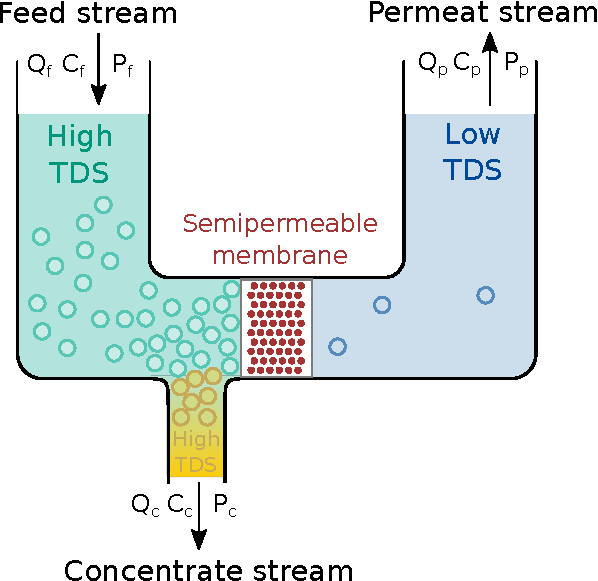
\includegraphics[width=0.4\textwidth]{Reverse_Osmosis}
% 	\caption[Reverse Osmosis schematic separation process]{Reverse osmosis schematic separation process. Based on: \cite{crittenden_mwhs_2012}.}
% 	\label{fig:ro}
% \end{figure} 

% The minimum energy required to push the water through the membrane is given by the amount of diluted solutes in the \textit{feed (f)} water. Such minimum energy can be estimated calculating the osmotic pressure of the \textit{feed} water, as described in \eref{eq:6} \cite{crittenden_mwhs_2012}.

% \begin{equation}\label{eq:6}
% \pi = \phi\cdot C\cdot R\cdot T
% \end{equation}

% \noindent{Where}:
% \begin{itemize}[label={-}]
% 	\item $\pi$: osmotic pressure (bar),
% 	\item $\phi$: osmotic coefficient, close to 1 (-), assumed a 0.95 \cite{crittenden_mwhs_2012},
% 	\item $C$: concentration of all solutes (mol/L),
% 	\item $R$: universal gas constant, 0.083145 (L$\cdot$bar/mol$\cdot$K),
% 	\item $T$: absolute temperature (K), (273 + \degree C), assumed at 25 \degree C for the entire aquifer.
% \end{itemize}

% Thus, the minimum energy demand can be estimated multiplying the osmotic pressure of the \textit{feed} water $\pi$ (in bar) by a conversion factor of 1.0 kWh/m\textsuperscript{3} = 36 bar. In reality, the energy demanded is greater due to factors as friction losses, membrane filtration resistance, among others. However, this approach has been used in cases were no specific data of the RO system is available \cite{KARABELAS201815}.

% The water quality layer used, was obtained from 206 measurements provided by National Authorities of the region. Each point specifies the spacial location and groundwater TDS content. Although the data did not covered the entire basin area, due to lack of any other related information it was used to produced a raster layer. An inverse distance weighted interpolation method, having as distance weighting factor an inverse distance to a power of 2 and a global search radius with maximum number of nearest points of 10 was used (see \fref{fig:TDS}).

% \begin{figure*}[!ht]
% 	\centering
% 	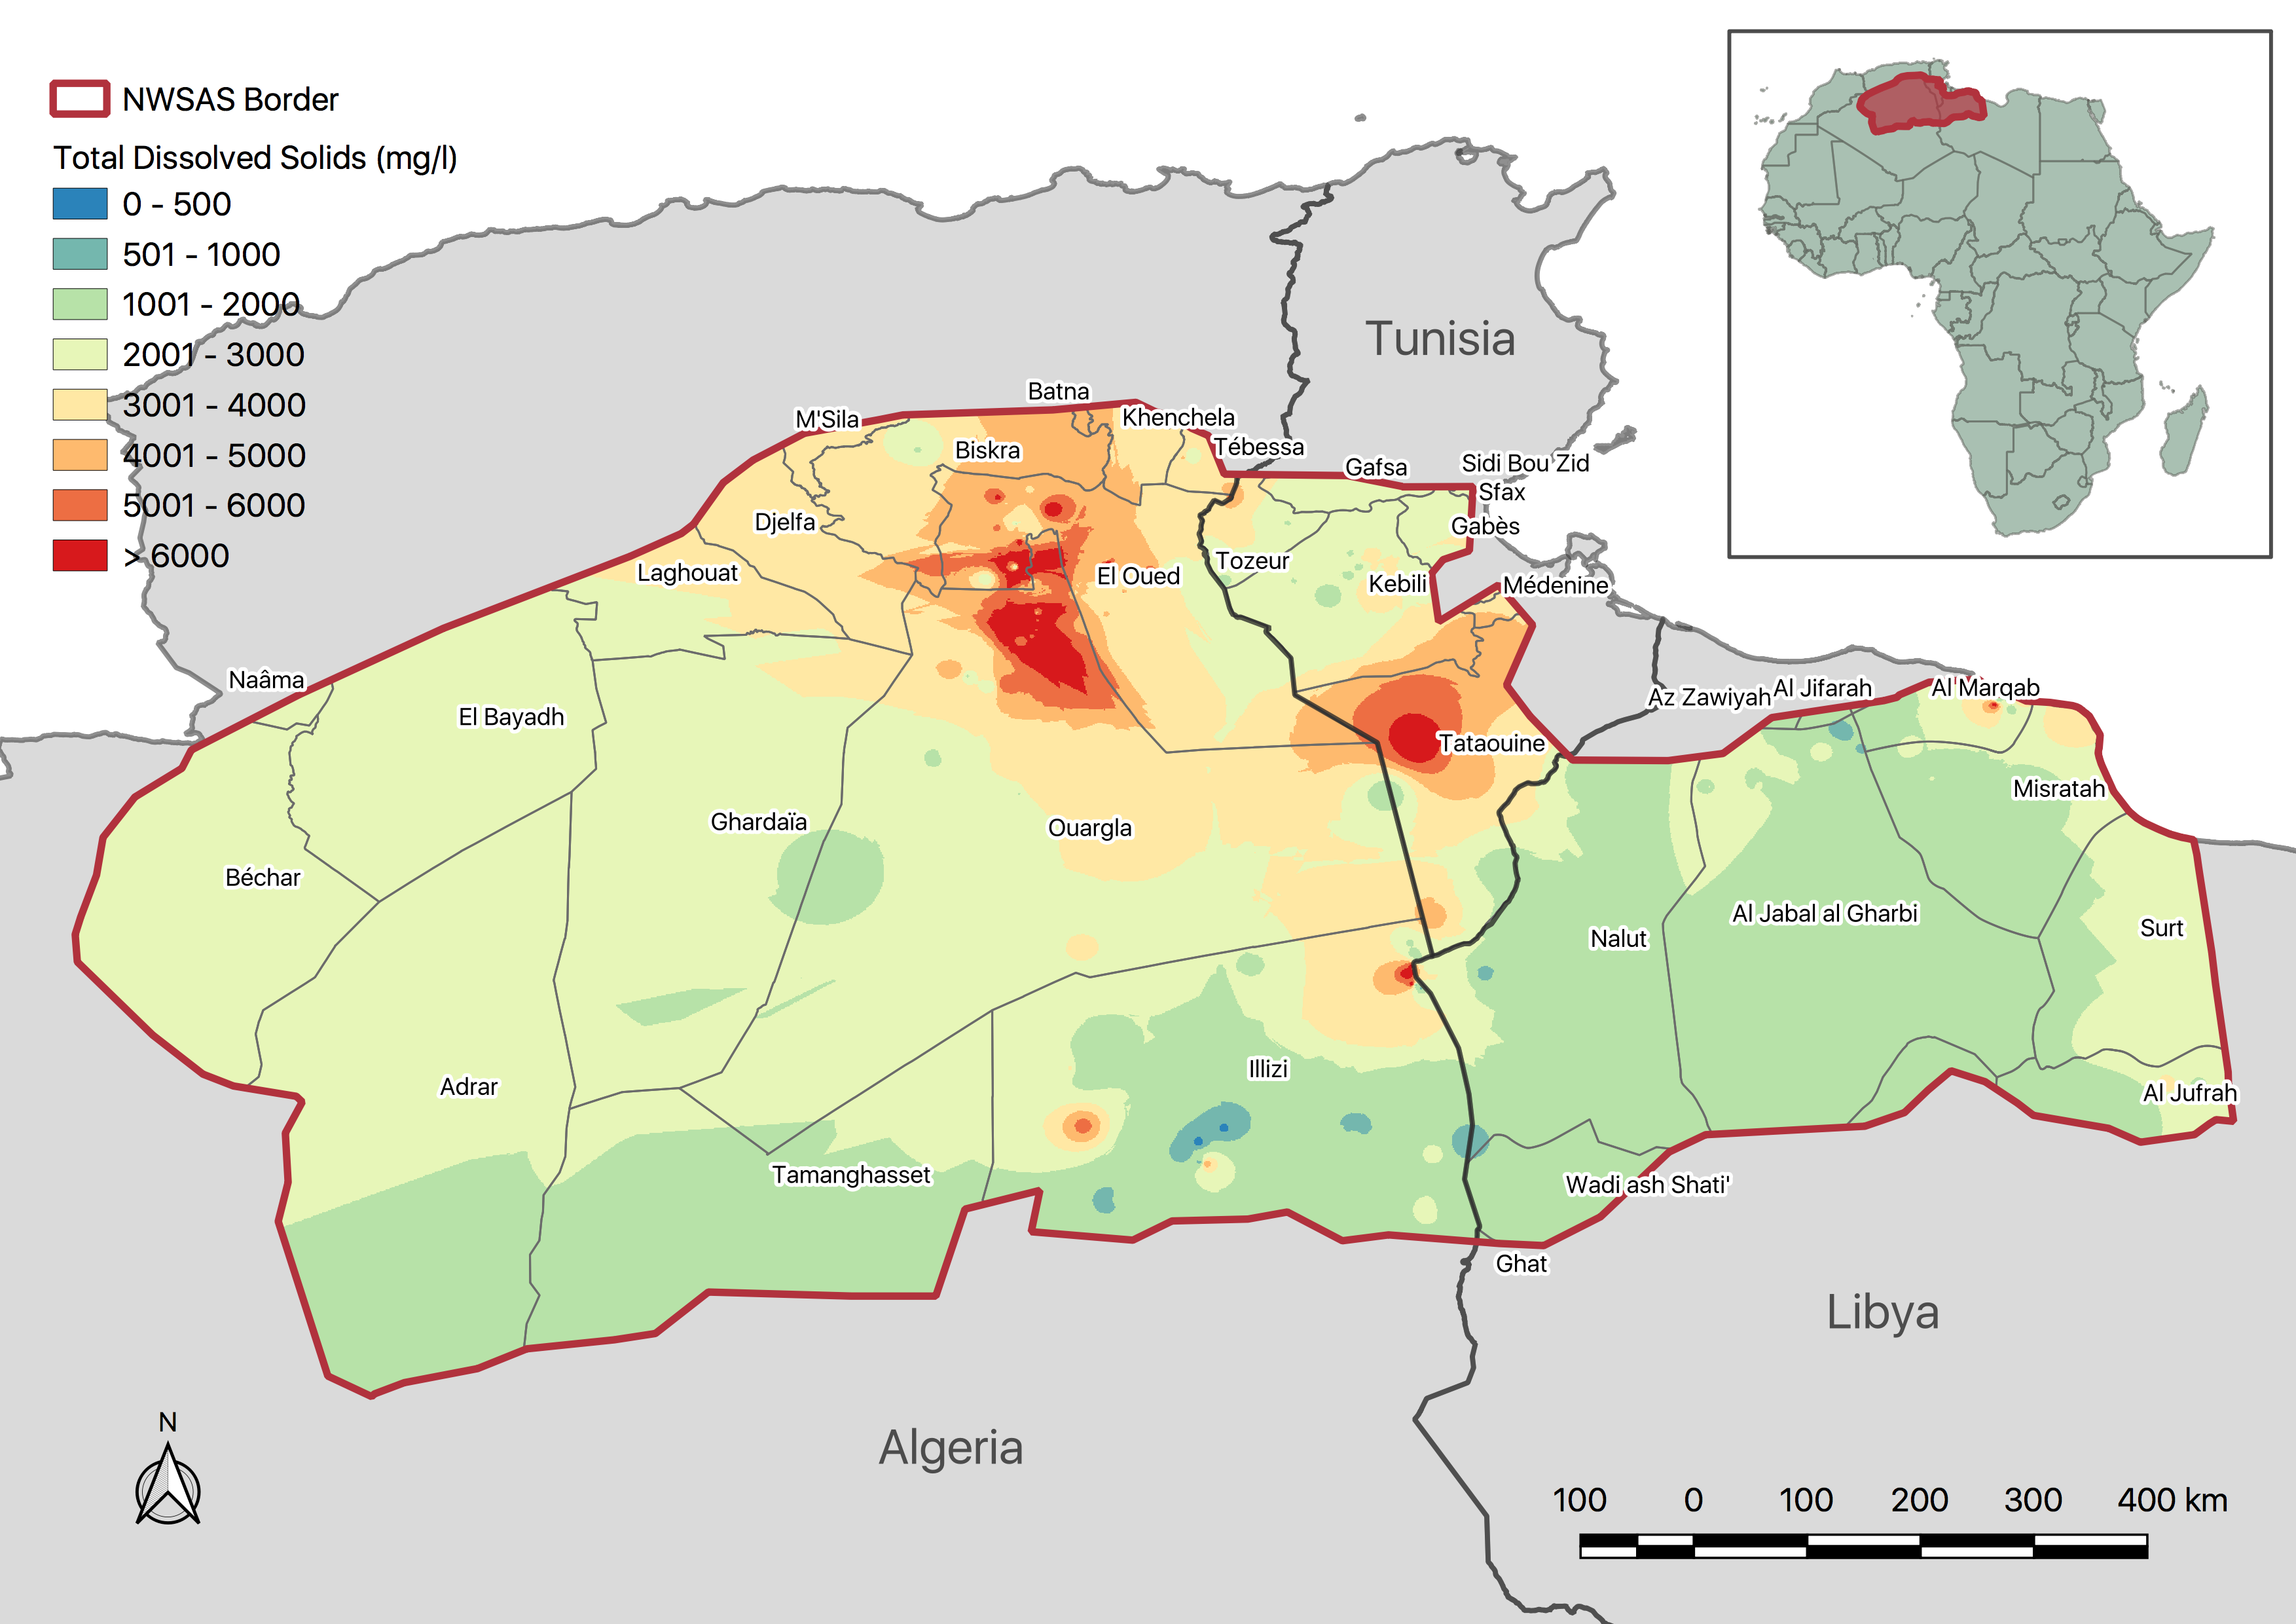
\includegraphics[width=0.88\textwidth, cfbox=black 1pt 0pt]{NWSAS_TDS}
% 	\caption[NWSAS groundwater quality map - Total Dissolved Solids (TDS)]{North Western Sahara Aquifer System - Groundwater quality map, Total Dissolved Solids (TDS) at 1$\times$1 km grid cell resolution.}
% 	\label{fig:TDS}
% \end{figure*}

% \subsection{Energy-for-wastewater}\label{Sc:eww}
% To calculate the energy-for-wastewater requirements an energy intensity factor was used for each evaluated treatment technology following \eref{eq:energy-for-wastewater}.

% \begin{equation}\label{eq:energy-for-wastewater}
% E_{ww} = Q_{ww,yr}\cdot X_t
% \end{equation}

% Where $Q_{ww,yr}$ represents the yearly treated wastewater in m\textsuperscript{3}/yr, and $X_t$ the average energy demand of the specific WWTT $t$, to treat one m\textsuperscript{3} of wastewater (in kWh/m\textsuperscript{3}).

\subsection{Clustering algorithm}\label{Sc:clustering}
A clustering approach was used in order to identify dense areas where a WWTS could be implemented, minimizing constraints imposed by existent large distances among scatter population or irrigated lands. A hierarchical clustering  algorithm was run using the \textit{Agglomerative Clustering} object from the Python \textit{scikit-learn} package \cite{scikit-learn}.
% Such algorithm relies on a bottom-up approach to define the clusters, in which all data points are first identified as an individual cluster, to be then successively merged together. The linkage criteria used was the \textit{ward} linkage.

\subsection{Wastewater Treatment System characteristics}
% The costs incurred in the implementation of a WWTS, can be divided into three major groups: \begin{enumerate*}[label=\upshape(\arabic*\upshape)]
% 	\item CAPEX, \item OPEX and \item Conveyance or transport system costs.
% \end{enumerate*} The first two, account for capital and operation expenses, and the third one for implementation and operation of the wastewater transportation system. Due to the high complexity of evaluating the costs of a conveyance system, only CAPEX and OPEX costs were considered.

% Statistical methods have shown to be commonly used among cost-modelling for wastewater management \cite{Costmodellingwastewater2011,Assessmentwastewatertreatment2012,Economicfeasibility2012}. Such methods use available cost figures (i.e. historical or estimated cost figures of actual WWTPs as capacity, pollutants treated, etc.) to create cost functions that adjust the cost relevant data to independent variables, describing the behaviour of a dependent variable (i.e. CAPEX and OPEX). The resulting cost function, allows to evaluate the capital and operational costs, often in terms of wastewater flow or served population equivalent \cite{Economicvaluationwastewater2015}. One advantage of this approach from a GIS perspective, is that with the use of non-linear cost functions, the effect of economies of scale can be easily evaluated. Furthermore, as a top-down approach enables for a better understanding of the relationship among variables and wastewater management, it constitutes a scientific approach for new wastewater services planning \cite{Costmodellingwastewater2011}. 

Wastewater pollutant levels, were assumed to be constant throughout the basin, using standard values based on studies from FAO \cite{fao1985water}. The assumed pollutant levels for population wastewater and the required levels for reused TWW, are shown in \tref{tbl:pollutans}.

% \begin{table*}[!ht]
% 	\caption{\label{tbl:pollutans}Pollutant levels of wastewater and treated wastewater (mg/l).}
% 	\begin{indented}
% 	\item[]\begin{tabular}{@{}l r r}
% 		\br
% 		Pollutant type & Wastewater & Treated wastewater\\
% 		\mr
% 		Suspended solids ($SS$) & 900 & 100\\
% 		Nitrogen ($N$) & 40 & 10\\
% 		Phosphorus ($P$) & 20 & 2\\
% 		Biochemical Oxygen Demand (BOD\textsubscript{5}) ($BOD_5$) & 500 & 50\\
% 		Chemical Oxygen Demand ($COD$)& 500 & 50\\
% 		\br
% 	\end{tabular}
% 	\end{indented}
% \end{table*}

Statistical methods have shown to be commonly used in cost-modelling for wastewater management \cite{Costmodellingwastewater2011,Assessmentwastewatertreatment2012,Economicfeasibility2012}, thus, cost functions were used to estimate CAPEX and OPEX values for the different WWTT. However, technology specific cost functions were not available for the NWSAS basin area, nor statistical data to develop them. Therefore, based on the work of \citet{Assessmentwastewatertreatment2012} cost functions for different WWTT in Spain were used to evaluate the competence of selected technologies in the NWSAS (see \tref{tbl:treatmentsystems}). Energy intensity characteristics were added for each technology according to \cite{Energypatternanalysis2012,ComparativeAnalysisEnergy2017}.

% \begin{table*}[!ht]
    \caption{\label{tbl:treatmentsystems}Treatment systems analysed. Adapted from \cite{Assessmentwastewatertreatment2012} unless otherwise stated.}
	{\footnotesize
	\begin{tabular*}{\textwidth}{@{}P{1.9in} P{1in} P{2in} P{0.7in}}
    \br
    Technology & Contaminants & Costs \& Energy & Water\\
    \mr
    Pond System (PS) & N: 20–40 \newline P: 60–70 \newline COD: 60–96 \newline SS: 50–90 & CAPEX: $3897.7\cdot x^{-0.407}$ \newline OPEX: $5.543\cdot x + 3127.5$\newline **Energy: $0.19\cdot V$ & Irrigation tailwater\\
    Intermittent Sand Filter (ISF) & N: 65–95 \newline P: 75–99 \newline COD: 75–90 \newline SS: 85–95 & CAPEX: $2115.5\cdot x^{-0.399}$ \newline OPEX: $12.026\cdot x+3518.9$\newline **Energy: $0.2\cdot V$ & Population wastewater\\
    Trickling Filter (TF) & N: 35–50 \newline P: 35–55 \newline COD: 75–90 \newline SS: 50–90 & CAPEX: $12237\cdot x^{-0.87}$ \newline OPEX: $13.504\cdot x+6020$ \newline **Energy: $0.3\cdot V$ & Population wastewater\\
    Moving Bed Biofilm Reactor (MBBR) & N: 10–20 \newline P: 30–40 \newline COD: 20–40 \newline SS: 60–80 & CAPEX: $1187\cdot x^{-0.165}$ \newline OPEX: $12.794\cdot x+6031$\newline **Energy: $0.8\cdot V$ & Population wastewater\\
    Rotating Biological Contractors (RBC) & N: 20–80 \newline P: 10–30 \newline COD: 70–93 \newline SS: 75–98 & CAPEX: $6931.4\cdot x^{-0.383}$ \newline OPEX: $313.4\cdot x^{-0.435}$\newline **Energy: $0.8\cdot V$ & Population wastewater\\
    Membrane Bioreactor (MBR) & N: 50–90 \newline P: 20–70 \newline COD: 70–90 \newline SS: 85–99 & CAPEX: $5635.3\cdot x^{-0.352}$\newline *OPEX: $2.116\cdot V^{0.713}e^{1.51\cdot SS+0.037\cdot BOD}$\newline **Energy: $0.8\cdot V$ & Population wastewater\\
    Extended Aeration (EA) & N: 50–90 \newline P: 15–70 \newline COD: 70–90 \newline SS: 85–99 & CAPEX: $7946\cdot x^{-0.460}$ \newline *OPEX: $169.48\cdot V^{0.454}e^{0.61\cdot SS}$\newline **Energy: $0.6\cdot V$ & Population wastewater\\
    Sequencing Batch Reactor (SBR) & N: 55–90 \newline P: 25–70 \newline COD: 70–90 \newline SS: 85–99 & CAPEX: $8258.9\cdot x^{-0.407}$ \newline OPEX: $309.4\cdot x^{-0.389}$\newline **Energy: $1\cdot V$ & Population wastewater\\
    \br
    \end{tabular*}\\
	~* Taken from \cite{Costmodellingwastewater2011}\newline ** Based on \cite{Energyrequirementswater2012,ComparativeAnalysisEnergy2017}\newline $x$: population equivalent, $x=V\times1500/(400\times365)$, $V$: wastewater flow (m\textsuperscript{3}/yr)}
\end{table*}

\subsection{Levelised Cost of Water (LCOW)}
A proposed LCOW method was used as metric to compare cost-effectiveness among WWTTs. The LCOW assesses the life-cycle cost of delivering one unit (e.g. one cubic meter) of treated wastewater, based on all physical assets and resources required. This concept, is inherited from the LCOE methodology, which applies the same life-cost analysis for one unit of electricity output \cite{prospectscostcompetitive2013}. The LCOW method follows the logic of the LCOE method \cite{prospectscostcompetitive2013,GeospatialLevelizedCost2015}, with pertinent adjustments to the variables used in wastewater treatment systems. Then, the LCOW can be expressed as follows:

\begin{equation}\label{eq:lcow}
LCOW = LCOW_{Inv} + LCOW_{O\&M} + LCOW_{Ext}
\end{equation}

The expression presented in \eref{eq:lcow}, disaggregates the $LCOW$ (\$/m\textsuperscript{3}) value in three components: the cost components due to investment $LCOW_{Inv}$, operation and maintenance $LCOW_{O\&M}$ and externalities $LCOW_{Ext}$. As the CAPEX function comprises all investment components of a WTTP, it enables an easy calculation of the $LCOW_{Inv}$ for each WWTT and each region or cluster. \Eref{eq:lcow_inv} describes the process to calculate the $LCOW_{Inv}$.

\begin{equation}\label{eq:lcow_inv}
LCOW_{Inv} = \frac{Inv}{\sum_{t=1}^{T} V_{t}\cdot\gamma^{t}}\cdot\Delta
\end{equation}

Where $Inv$ stands for the CAPEX value, $V_{t}$ for the treated water flow per year $t$ (m\textsuperscript{3}/yr), $\Delta$ for the tax factor and $\gamma^{t}$ represents the discount factor of the project \eref{eq:gamma}. The discount factor can be calculated according to the discount rate $r$, as shown in \eref{eq:gamma}. An appropriate discount rate ($r$) needs to be used to ensure the right amount of return for all sources of long term capital (i.e. equity holders and debt). Often, the proper discount rate used is the WACC, which was assumed at 4\% for this study \cite{prospectscostcompetitive2013}. 

\begin{equation}\label{eq:gamma}
\gamma^{t} = \left(\frac{1}{1+r}\right)^{t}
\end{equation}

The tax factor $\Delta$ includes all effects of the tax related variables, these being the rent tax, depreciation, depreciation period, discount factor and investment tax credit \cite{prospectscostcompetitive2013}. No effects related to the tax factor were considered, thus a tax factor of $\Delta=1$ was used.

The LCOW related to operational costs $LCOW_{O\&m}$ \eref{eq:lcow_om} was computed by using the OPEX values $\omega_{t}$ calculated for each year in each cluster, the treated water flow $V_{t}$ (m\textsuperscript{3}/yr) and the discount factor $\gamma^t$ per year.

\begin{equation}\label{eq:lcow_om}
LCOW_{O\&m} = \frac{\sum_{t=1}^{T} \omega_{t}\cdot V_{t}\cdot\gamma^{t}}{\sum_{t=1}^{T} V_{t}\cdot\gamma^{t}}
\end{equation}

Furthermore, the avoidance of externalities due to discharge of untreated wastewater into ecosystems can be accounted in the LCOW calculation. This parameter tries to account for the effects that pollutants presented in wastewater and tailwater stream flows can have into fresh water bodies, rivers or groundwater aquifers \cite{Assessmentwastewatertreatment2012}. The externalities-related LCOW value $LCOW_{Ext}$ \eref{eq:lcow_ext} can be obtained as follows:

\begin{equation}\label{eq:lcow_ext}
LCOW_{Ext} = \frac{\sum_{p}^{P}\sum_{t=1}^{T} m_{p}\cdot B_p\cdot V_{t}\cdot\gamma^{t}}{\sum_{t=1}^{T} V_{t}\cdot\gamma^{t}}
\end{equation}

Where $m_p$ represents the concentration of pollutant of class $p$ avoided with the treatment of one cubic meter of wastewater (kg/m\textsuperscript{3}), and $B_p$ the environmental benefit of avoiding one kilogram of pollutant $p$ running into the environment (\$/kg). Unfortunately, due to lack of information of environmental effects of wastewater pollutants in the region, this parameter was not considered.

Finally, the project life span was set for 35 years, having as starting year 2015 and ending year 2050.

% \subsection{Least-cost option}
% After the LCOW values were calculated, the WWTT with the lowest $LCOW$ value for each cluster was identified.

\section{Results}
As described in the methodology section, a clustering approach was used to minimize the constraints imposed by scattered and distant population and cropland points. Forty clusters were created (\Fref{fig:clusters}) in the process, which succeeded in identifying dense agglomerations. When compared with a traditional approach of performing an analysis on a province basis, the clusters achieved a reduction of 347\% on the overall distance between points.

\begin{figure*}[!h]
    \centering
	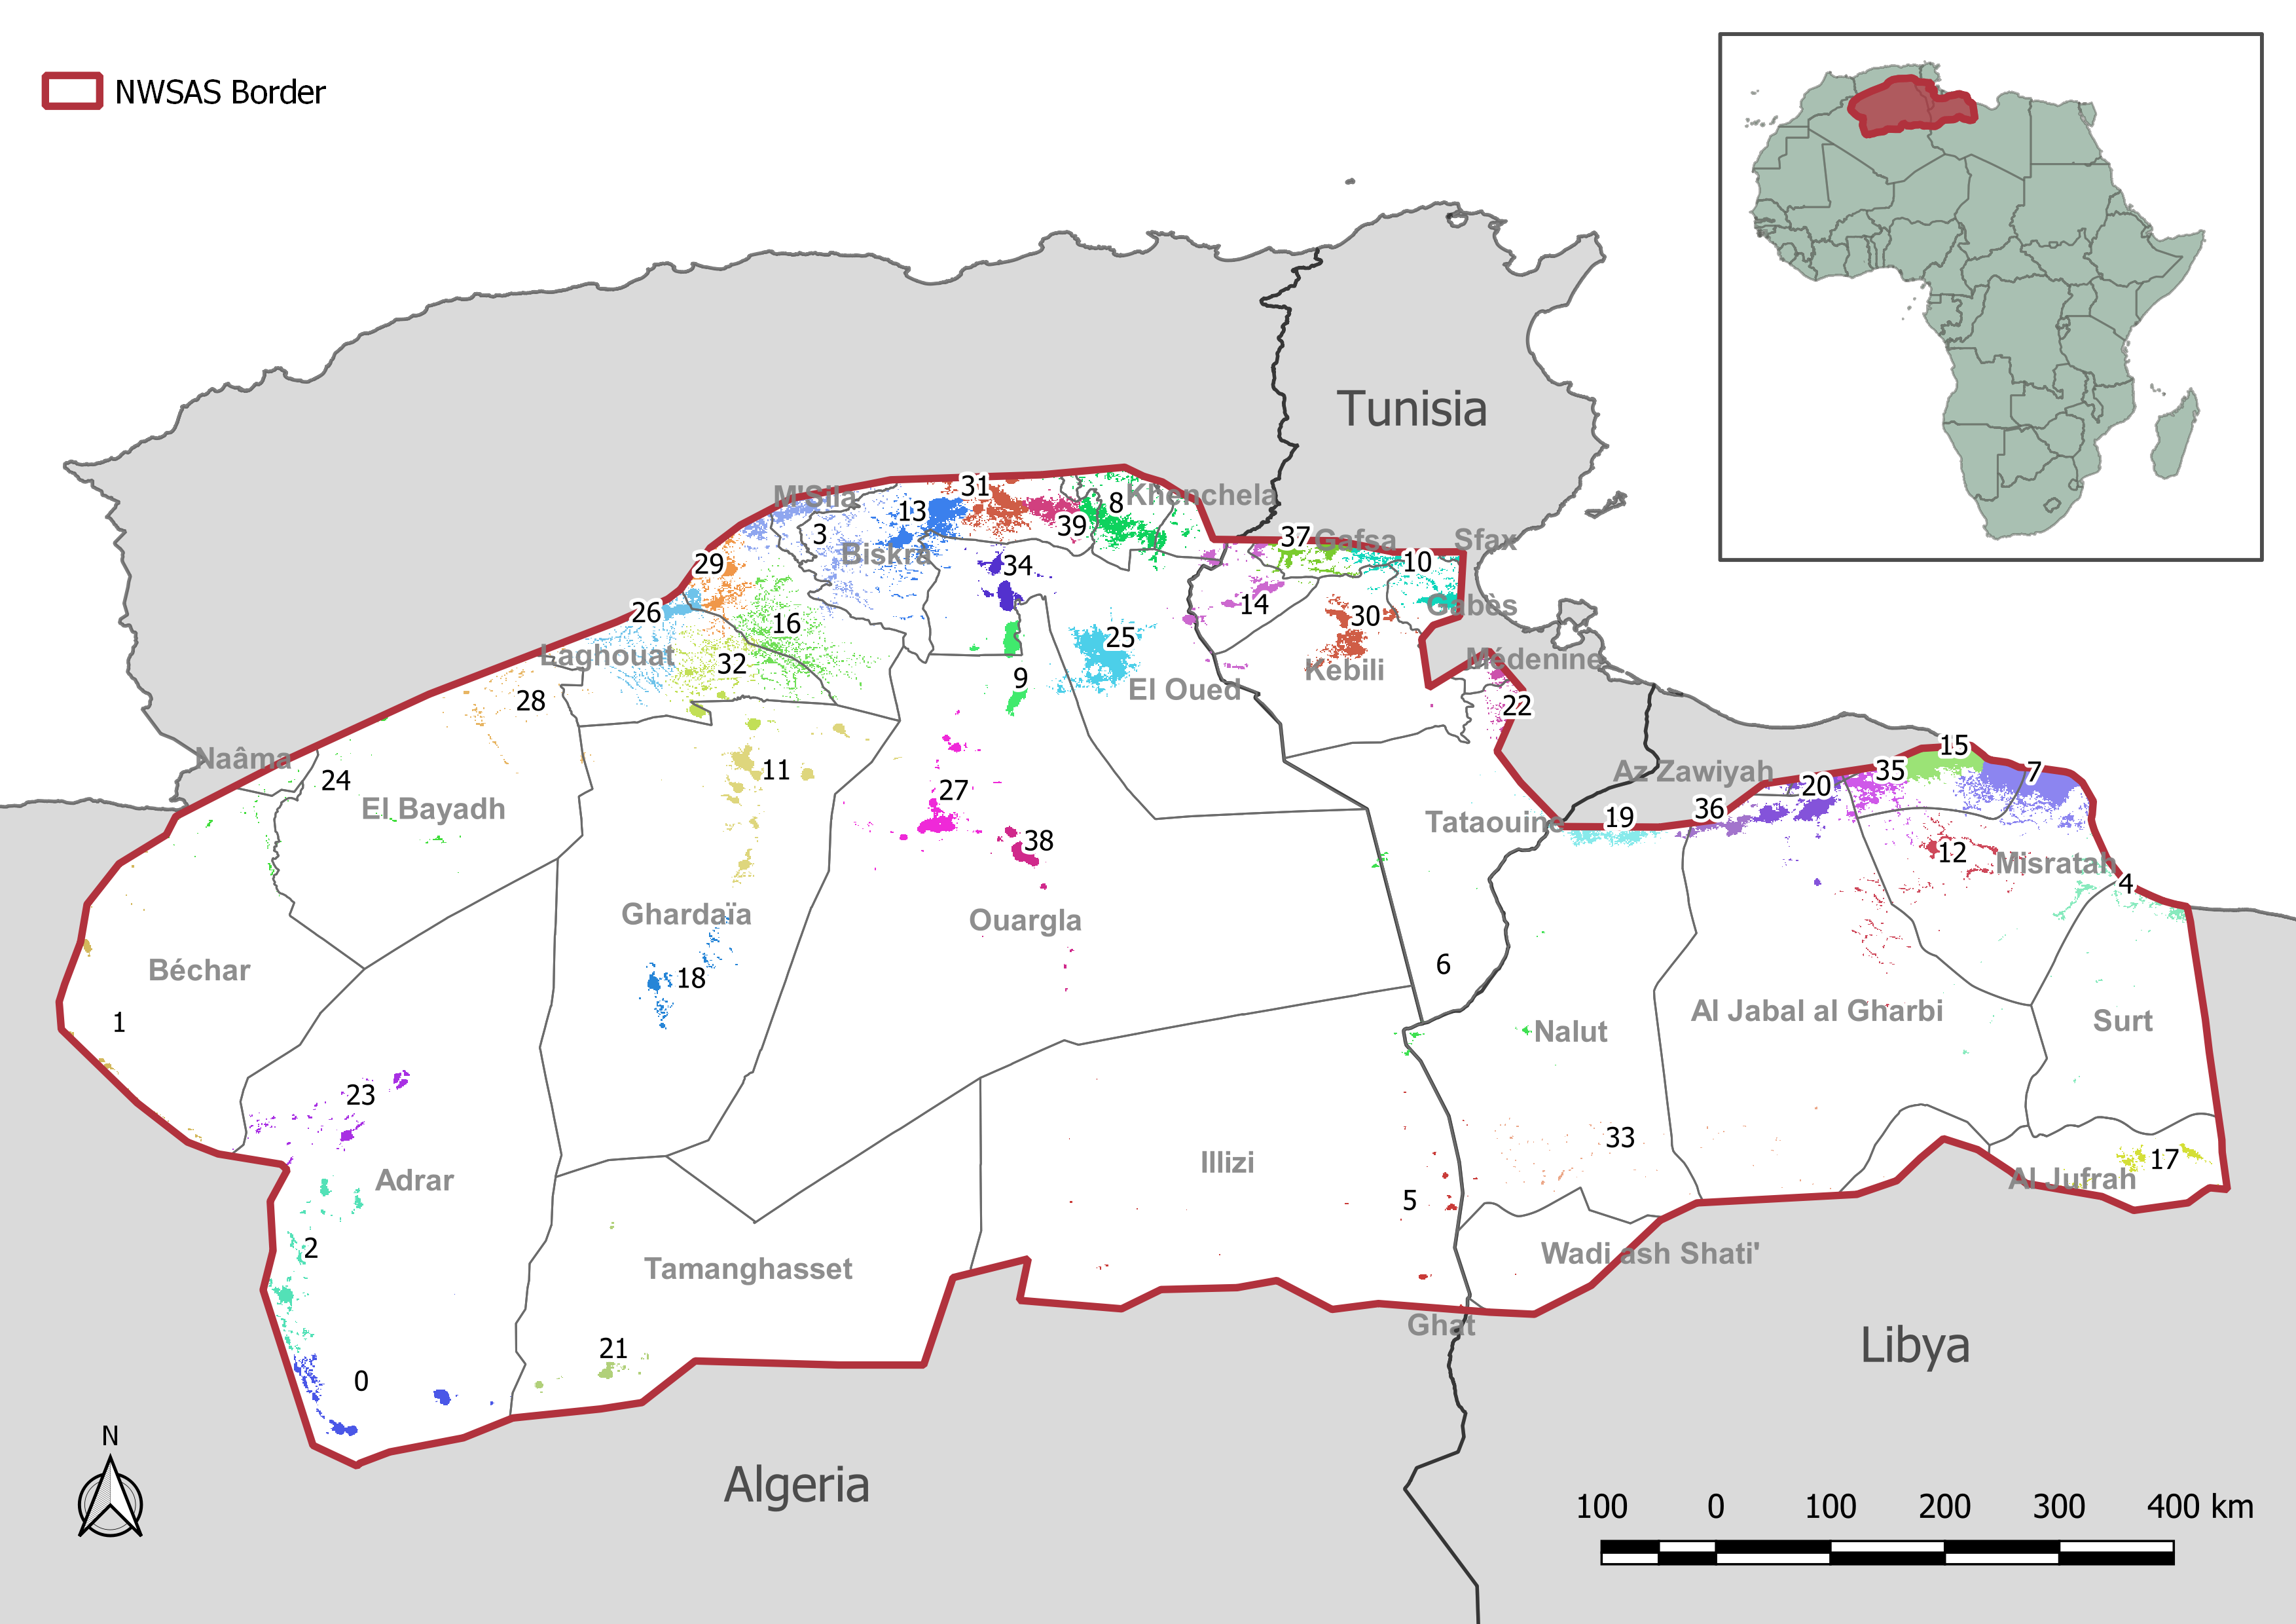
\includegraphics[width=0.88\textwidth, cfbox=black 1pt 0pt]{NWSAS_clusters}
	\caption{Population and cropland clusters. Clusters are numbered from 0 to 39, yielding 40 agglomerations including each population and cropland areas. Every cluster is tagged with a number and colored to make them stand out from others. The grey administrative boundaries correspond to the different provinces.}
	\label{fig:clusters}
\end{figure*}

This is especially important in larger provinces with important population and agricultural activity as Adrar, Ghardaïa, Ouargla el Oued and Misratah. Moreover, with this approach, the administrative border constraint is eliminated, as can be seen with cluster number 9 where the agglomeration shares areas from the Ouargla and El Oued provinces. This implies an interesting question for the need of collaboration between provinces and even countries.

Water use in the Baseline scenario was estimated at 5,913 Mm\textsuperscript{3}/yr, agricultural irrigation accounting for 94\% share (see \fref{fig:water}). In the water reuse scenario with private agricultural water regime, the overall water use was lower than the baseline, opposite behaviour to the subsidized and free agricultural water schemes. However, due to the reused water share in the subsidized regime, the overall water extractions were lower than those of the Baseline and close to the ones from the private regime. This suggests that either with the use of more efficient irrigation schemes (i.e. the private regime) or the use of lower efficiency irrigation coupled with water reuse (i.e. subsidized regime), similar results could be achieved.

\begin{figure*}[!ht]
	\centering
	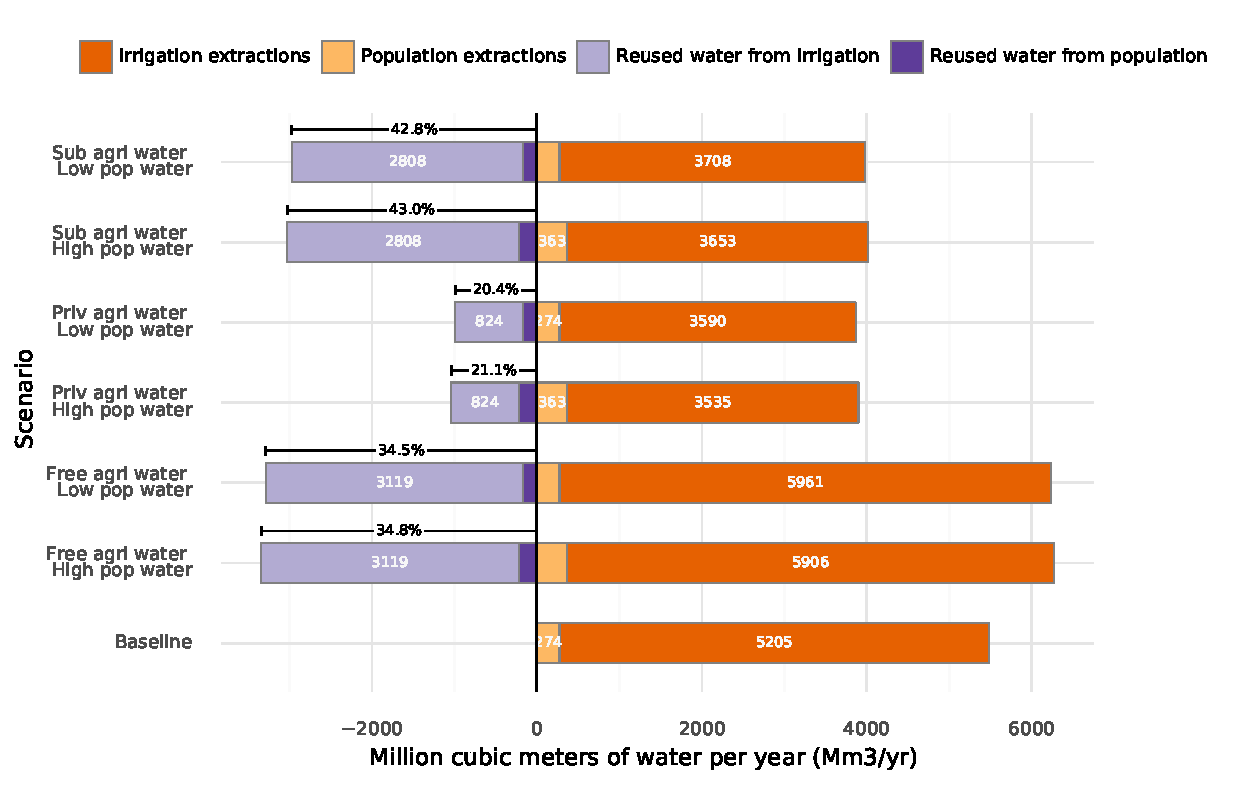
\includegraphics[width=\textwidth]{Water}
	\caption{Water usage for all scenarios. At left: reused water after reclaim, treatment and allocation classified by population and irrigation source. At right: overall water extractions classified by population and irrigation use. Percentage bars indicate the share of reused water against the total demand.}
	\label{fig:water}
\end{figure*}

On the other hand, the free agricultural water regime yielded much larger water extractions, even with water reuse. In fact, the share of reused water accounted for around 34\% of the water usage, lower share than that of the subsidized regime. This was due to the cap set to the on-farm storage area of maximum 2\% share of the cropland area. Therefore, while more recoverable water is available in the free water regime, the storage system cannot hold everything. This could be solved by setting a higher value for the permissible on-farm storage area, however, this would mean that more agricultural area would be lost for storage purposes which can affect the farmers' revenues.

Population water levels do not cause meaningful variations in the overall water use, as agricultural water needs are much more extensive. Nonetheless, with the use of more efficient irrigation schemes, the recoverable water from irrigation drainage decreases, thus populations treated wastewater share on agricultural water usage increases.

The Groundwater Stress Indicator was computed aggregating the entire aquifer area (\fref{fig:gws}). A value of 5.36 in the Baseline scenario was obtained, which falls inside the medium to high stress category---however, it is known that the stress level in some parts of this area can reach to the extremely high category \cite{herbertGlobalAssessmentCurrent2019}. The private and subsidized agricultural water scenarios, presented a Groundwater Stress Indicator in the category of low to medium stress, which suggests a success by the treated wastewater measure in reducing the stress on the resource. However, the outcomes obtained for the free agricultural water scenarios, are higher at 5.72 and 5.77. Such increase in the stress, is due to the higher water requirements for agricultural irrigation, which suggest that the treated wastewater measure would not be enough for reducing the overall water stress on the aquifer, if it is not accompanied by water management and proper pricing mechanisms, that ensure the appropriate use of the resource by local farmers.

\begin{figure}[!h]
	\centering
	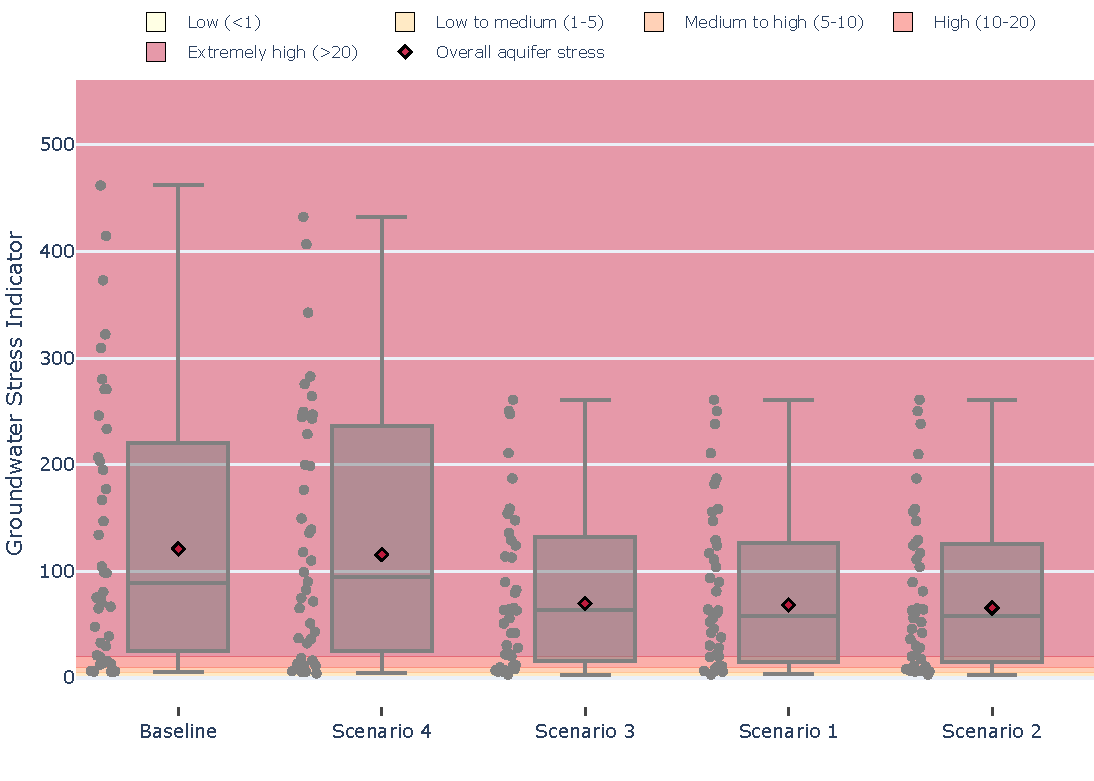
\includegraphics[width=0.7\textwidth]{GWS}
	\caption{Groundwater stress indicator for all scenarios.}
	\label{fig:gws}
\end{figure}

The least-cost treatment systems obtained for the low and high population water scenarios, share similarities in the combination of technologies identified (\fref{fig:leastLow} and \fref{fig:leastHigh}). Extended aeration, rotating biological contractors and intermittent sand filter were the least-costly technologies chosen. Nonetheless, differences in the technology shares exist. In the low population water requirements scenarios, wastewater was treated by intermittent sand filters, rotating biological contractors and extended aeration by 4\%, 21\% and 75\% share respectively. Whereas, in the high population water requirements scenario this shares were 2\%, 11\% and 87\%. In general, when lower capacity is required simpler treatment technologies are more cost-effective, as the independent variable of the CAPEX and OPEX cost functions is the available reclaimed wastewater flow.

\begin{figure*}[!ht]
	\centering
	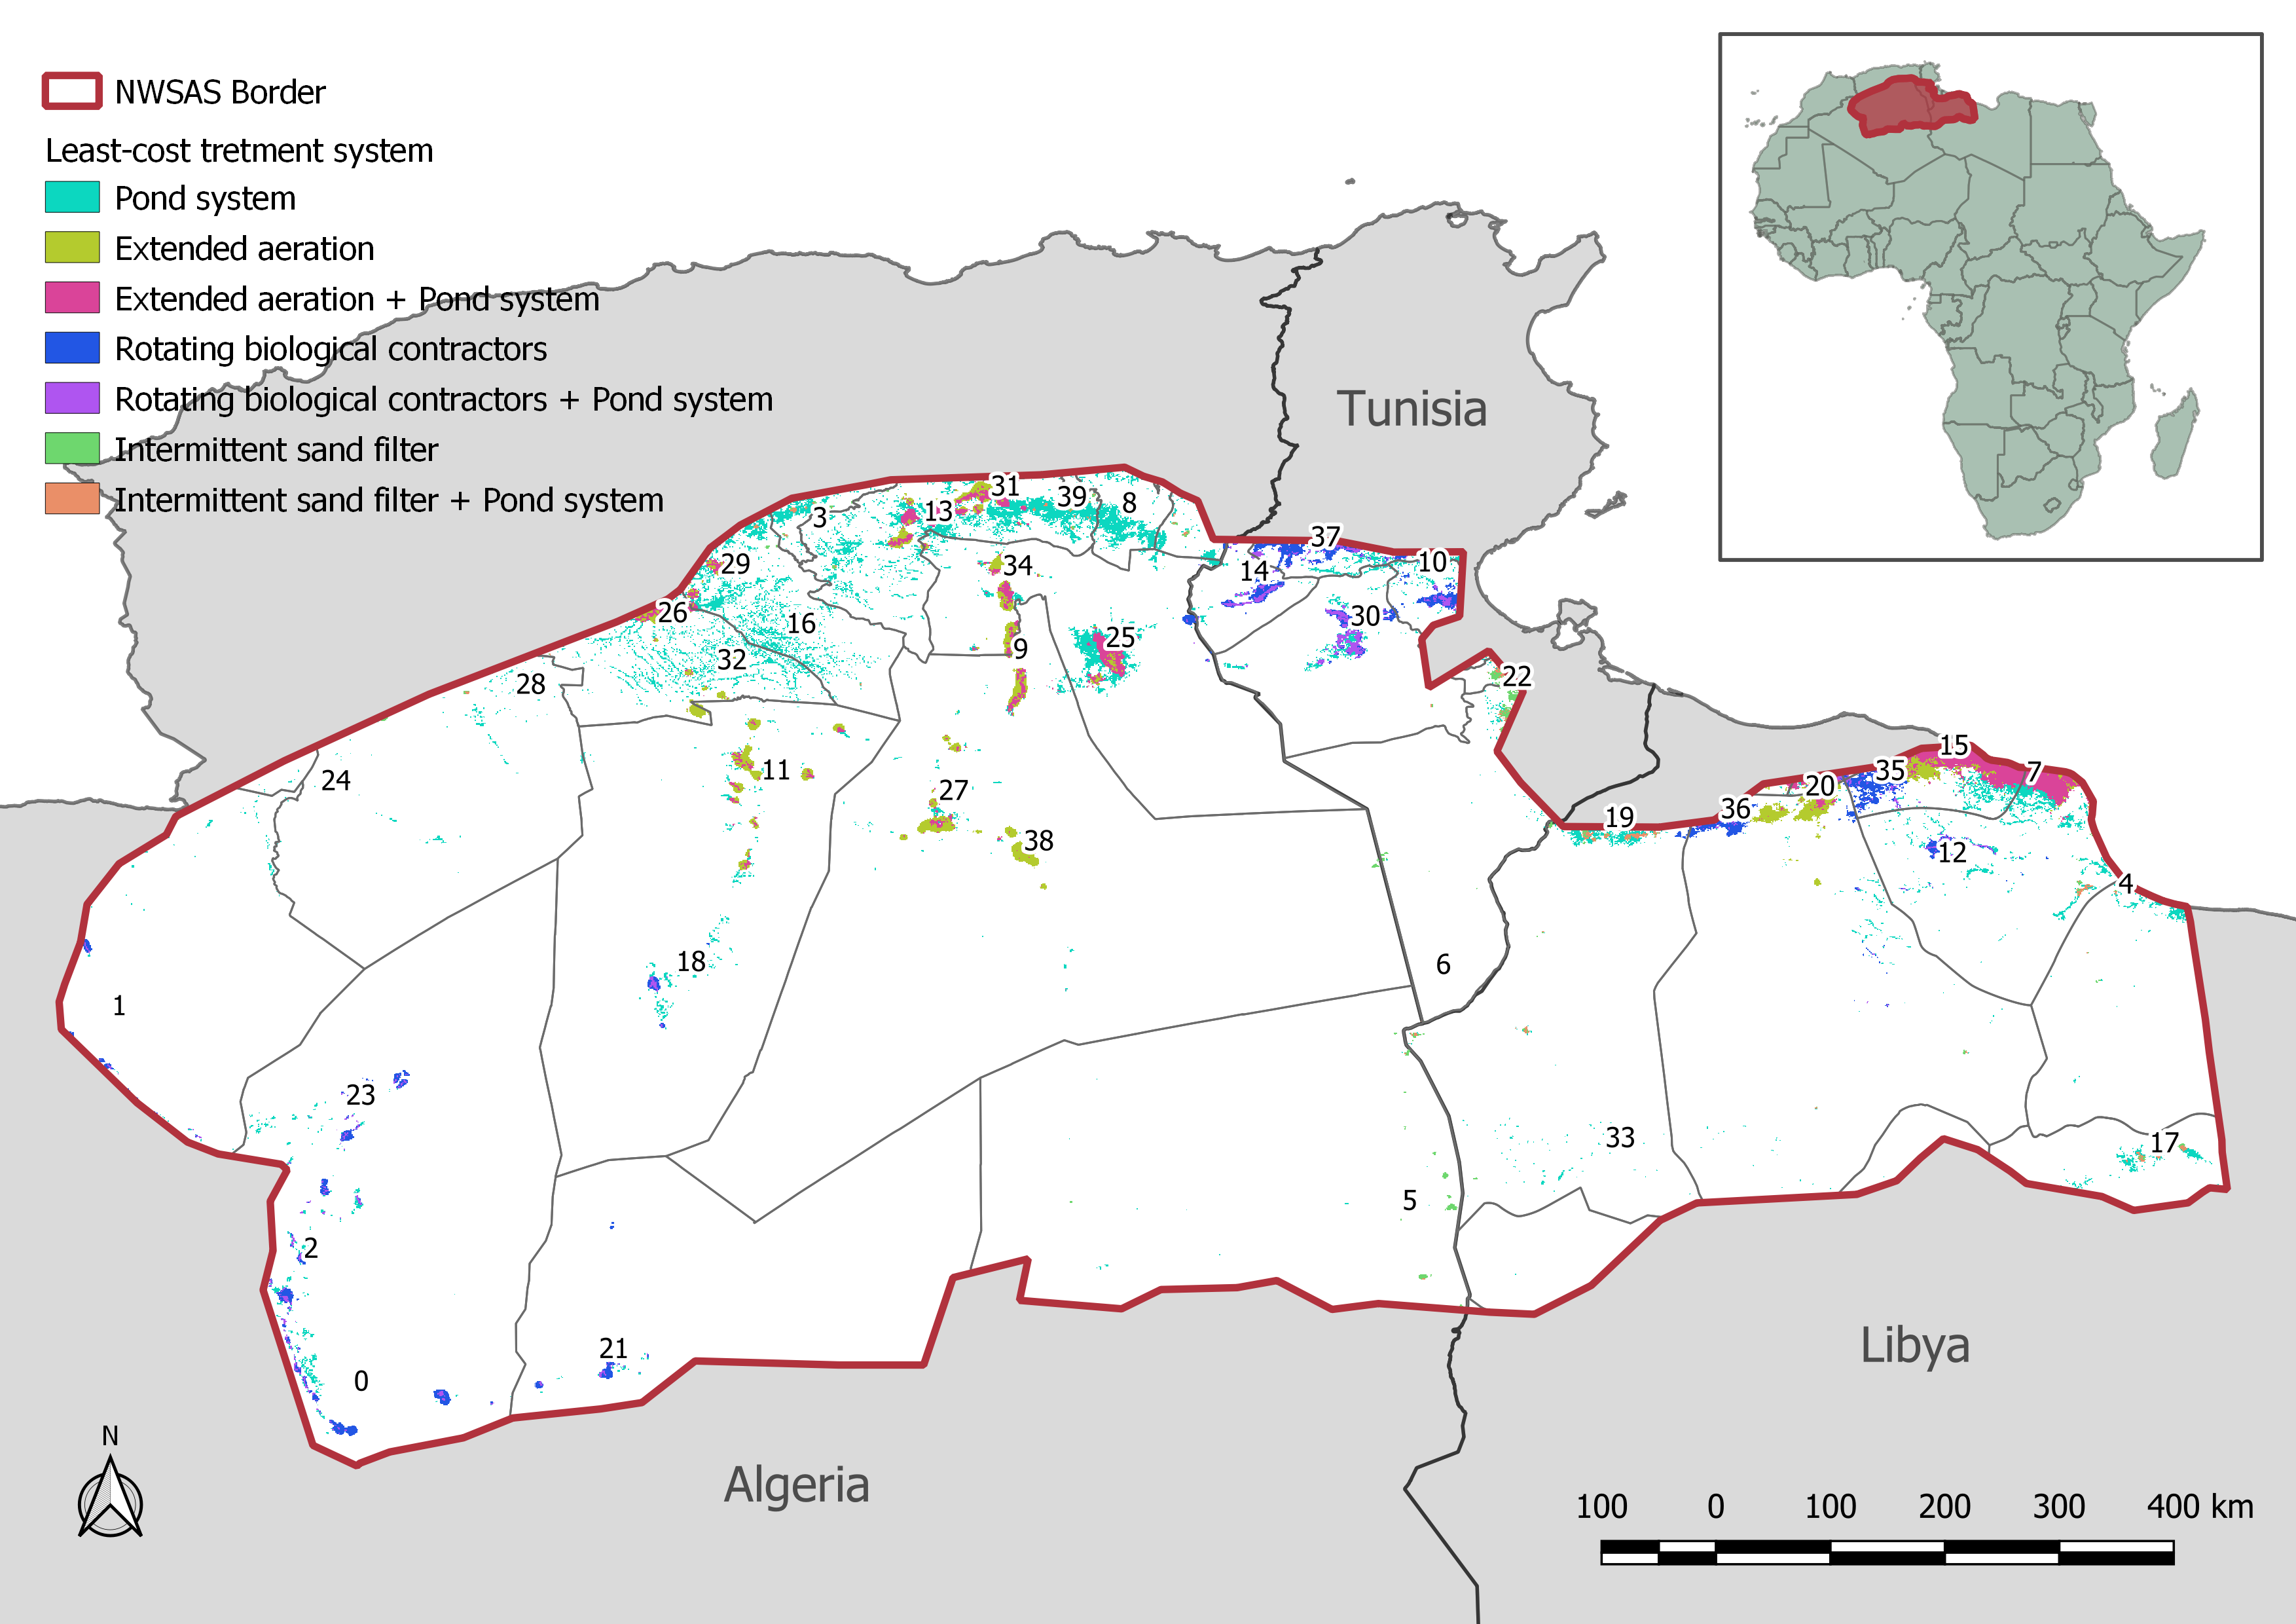
\includegraphics[width=0.88\textwidth, cfbox=black 1pt 0pt]{NWSAS_least-cost_system_cluster}
	\caption{Least-cost wastewater treatment options per cluster---low population water requirements.}
	\label{fig:leastLow}
\end{figure*}

\begin{figure*}[!ht]
	\centering
	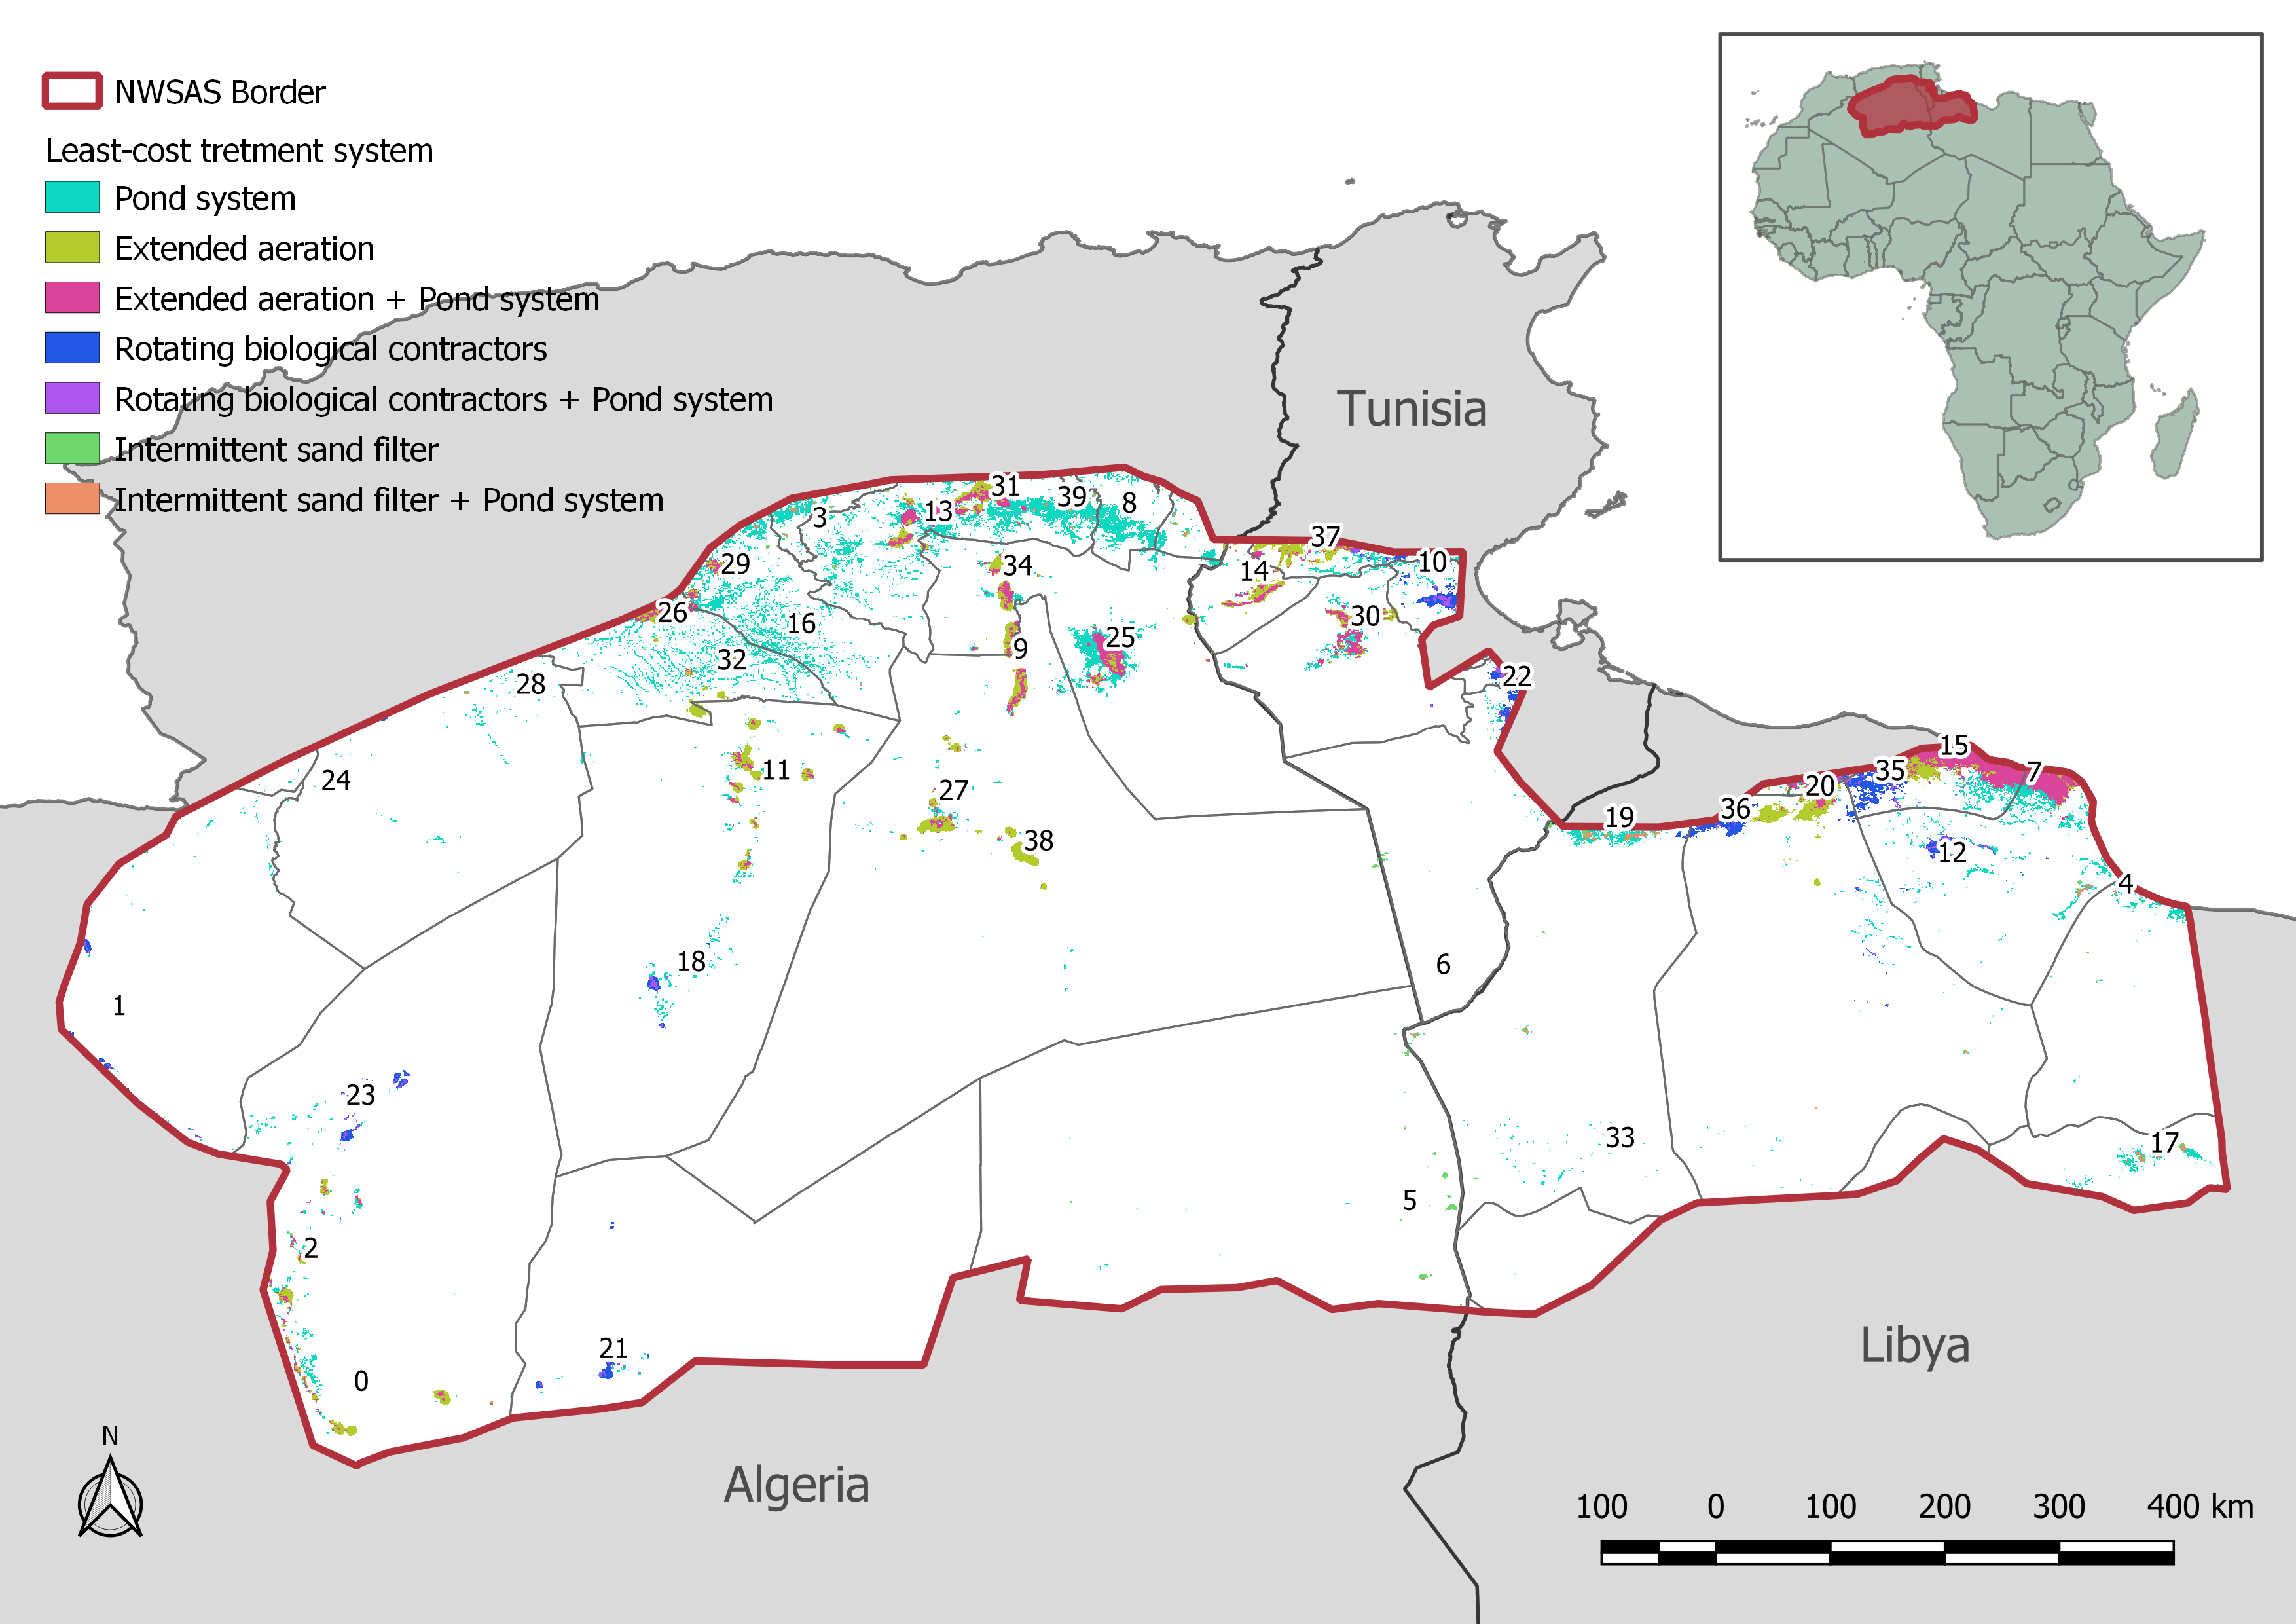
\includegraphics[width=0.88\textwidth, cfbox=black 1pt 0pt]{NWSAS_least-cost_system_cluster_high}
	\caption{Least-cost wastewater treatment options per cluster---high population water requirements.}
	\label{fig:leastHigh}
\end{figure*}

The previous is important, as the amount of wastewater available from the agglomerations is key for the calculation of the least costly technology. Therefore, with larger agglomerations, scalable and higher capacity systems could be implemented. The downside however, is that if the costs related to the conveyance system are not evaluated, then the distances among population and/or irrigation points become irrelevant, which is arguably far from reality. Thus, the analysis of more compact clusters, reduces the drawbacks of not calculating the costs related to a wastewater conveyance system.

Overall, the least-cost treatment systems obtained, show an important trade-off, as the best solution is dependent from geospatial factors than can render a specific technology less costly than other in a given region. For example, clusters 0, 2, 37, 30 and 14 use rotating biological contractors in the low population water requirements scenarios, whereas extended aeration in the high population water scenario. Similarly, cluster 22 passes from using intermittent sand filters to biological rotating contractors.

\begin{figure*}[!b]
	\centering
	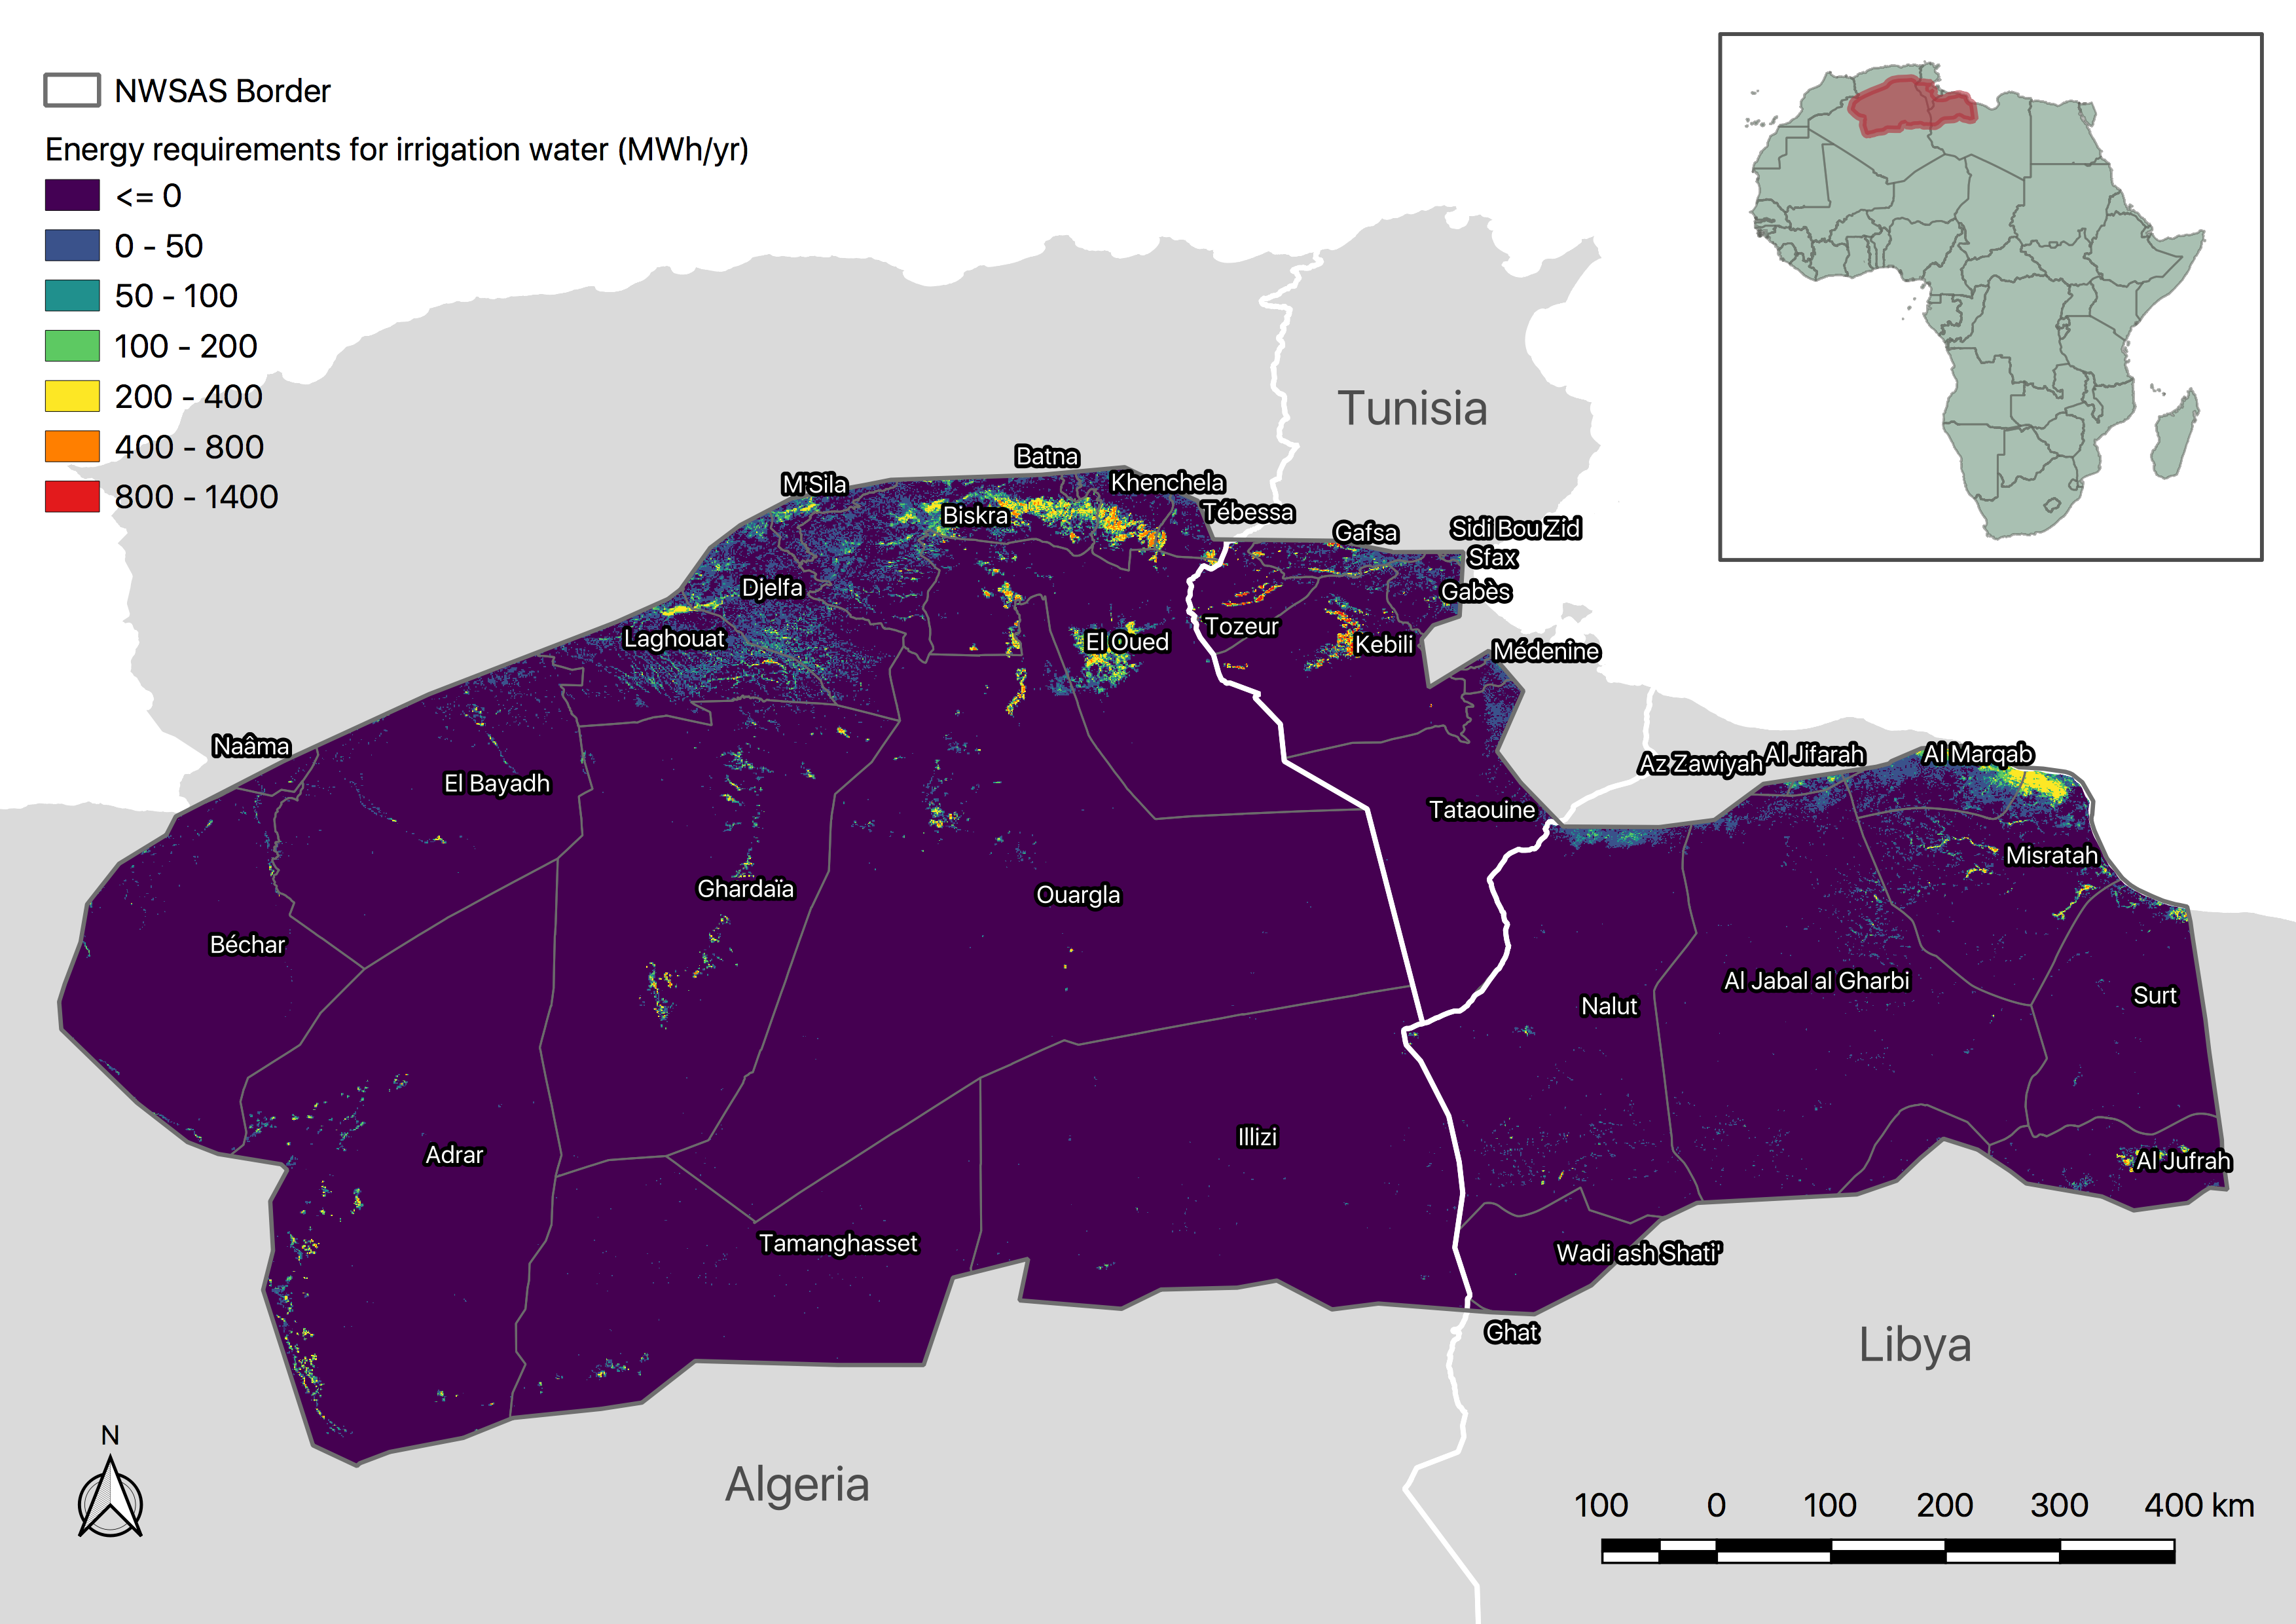
\includegraphics[width=0.88\textwidth, cfbox=black 1pt 0pt]{NWSAS_Energy_map}
	\caption[NWSAS energy used for irrigation water map - Baseline scenario]{North Western Sahara Aquifer System - Energy used for irrigation water map - Baseline scenario.}
	\label{fig:energy_map}
\end{figure*}

Yearly pumping energy requirements for agricultural water are shown in \fref{fig:energy_map}. The energy demand is considerably larger for Algeria and Tunisia in the northern parts of the aquifer. This is due to the higher average water demand per hectare existent in Algerian and Tunisian (according to statistics), the higher salinity contents found in this areas and the intense agricultural activity. On the other hand, the Al Marqab and Misratah provinces in Libya, present medium range energy consumption, even though the agricultural activity there is considerably high. Moreover, the energy needs for agricultural irrigation in the Adrar province, are in the medium to high range, although cropland density is much lower compared to the northern provinces. This suggests that, the deeper water table levels found along the province, can significantly affect the pumping energy requirements, impacting as well the water productivity of the region.

The overall energy related outcomes for all scenarios are shown in \fref{fig:energy}. The energy requirements for groundwater pumping represent the major part of all three activities. Desalination energy, although considerable, is much smaller than pumping energy, this mainly due to the medium TDS levels found throughout the groundwater aquifer. All scenarios apart from the free agricultural water ones, reduced overall energy consumption compared to the Baseline. Such reductions, are achieved by the reuse of treated wastewater in irrigation, as the energy intensity of treatment is substantially lower than the energy intensity for pumping water from the deep aquifer.

\begin{figure*}[!ht]
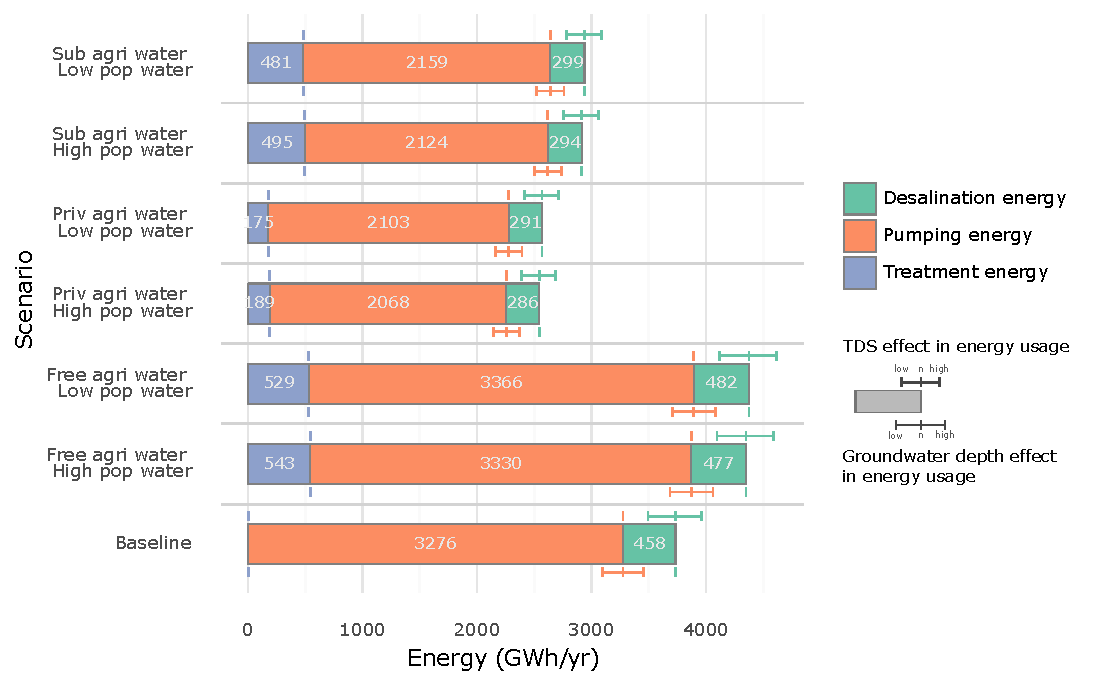
\includegraphics[width=\textwidth]{Energy}
\caption{Energy requirements for all scenarios with TDS and groundwater depth sensitivity analysis. TDS levels correspond to: $low=0.5\times n$ and $high=1.5\times n$; and groundwater depth levels correspond to: $low=n-10$ and $high=n+10$ meters.}
\label{fig:energy}
\end{figure*}

The sensitivity analysis demonstrates how a change of \rpm10 meters in the depth to groundwater level, has an average variation of circa \rpm5.5\% over the overall pumping energy requirements. Moreover, desalination energy requirements showed variations of $-$53\% to $+$50\%, when changes of \rpm50\% in the TDS levels were considered.

These effects on the energy-for-water requirements, are necessary to be assessed when planning for new water policies and water management strategies. Accordingly, accounting for new energy infrastructure, or potential energy savings could be key for the success of a new policy or solution to the water scarcity problem.

\section{Discussion and broader sustainable development implications}
Wastewater reclaim, treatment and reuse, has a clear potential to alleviate water stress in the NWSAS, while supporting sustainable food production and energy efficiency. By using a nexus approach, the synergies between SDGs targets can be easily analysed, facilitating and guiding sustainable development in the region. Wastewater treatment and reuse can indirectly improve water supply (SDG 6.1), as it increases water availability. Water quality (SDG 6.3) is directly enhanced and water efficiency (SDG 6.4) clearly improved as shown by the groundwater stress indicator. Food security (SDG 2.1/2.2) and agricultural production are directly supported by the reuse of nutrients present in treated wastewater, as well as by adopting sustainable practices (as tailwater reclaim and treatment) and reducing soil salinization (due to reduction of untreated wastewater/tailwater discharged to the environment). Energy efficiency (SDG 7.3) can be positively affected, as wastewater treatment showed to be less energy intense than pumping water from the groundwater aquifer. Thus, by reusing treated wastewater the overall use of energy per cubic meter delivered could be reduced. This, however, is dependent on the wastewater reclaim and treated wastewater supply system. If large centralized systems are implemented, the need to cover long distances from supply to demand may be inevitable (i.e. wastewater collection points to agricultural irrigation sites), thus large amounts of energy may be required for surface water pumping. Nonetheless, by using decentralized systems (e.g. on-farm treatment and wastewater treatment in small agglomerations), those issues can be lessen. Renewable energy share (SDG 7.2) can be positively affected too, as with modern wastewater treatment systems with on-site energy generation (e.g. biogas capture from sludge), large parts of wastewater treatment energy requirements can be provided, increasing the overall share of renewable energy. Moreover, by supplying treated wastewater to farmers, on-farm pumping from groundwater aquifers can be reduced, reducing as well the use of fossil fuels and electricity from the grid---the electricity generation mix in the NWSAS countries is heavily dominated by fossil fuel sources, making it an unclean source of energy \cite{AlgeriaElectricityHeat2016,LibyaElectricityHeat2016,TunisiaElectricityHeat2016}. Accordingly, climate mitigation can also be improved as both the water and the agricultural sectors GHG emissions would be reduced. Moreover, climate resilience (SDG 13.1) also has potential to be improved, as the increase on water availability for agricultural production (and indirectly for drinking purposes), would aid on severe drought periods. Synergies with SDG 8, SDG 12, income opportunities, employment opportunities and human well-being could also be found. This was argued by \citet{hoffNexusApproachMENA2019}, who covered 2 case studies of wastewater reuse in the MENA region and identified similar synergies as the ones previously presented.

Despite the synergies and high potential treated wastewater has in supporting sustainable development and alleviate water scarcity, it can be argued it is not enough. This is supported by the modelling results presented, as non of the scenarios achieved a substantial reduction on groundwater stress. In fact, one of the main parameters affecting such indicator was the water use behaviour of farmers towards price regimes. The inappropriate valorization of water in the NWSAS has been already identified, as well as the inefficiency of irrigation \cite{BetterValorizationIrrigation2015}. Therefore, water management strategies and proper pricing mechanisms that ensure the appropriate use of the resource by local farmers are needed. Moreover, the perception of wastewater reuse from local farmers is key on achieving successful strategies, as in some cases this has shown to be an important barrier for treated wastewater reuse \cite{mahjoubPublicAcceptanceWastewater2018}. As \citet{mahjoubPublicAcceptanceWastewater2018} analyse ``aspects related to education, knowledge, risk perception, culture, regulation, and communication need to be seriously addressed for a more viable and efficient use of wastewater in agriculture".

There is great value on having a Nexus approach while evaluating the treated wastewater reuse measure. It enables to identify and potentiate synergies and mitigate or avoid trade-offs. Nexus thinking has the potential to enhance well-being by decoupling it from natural resources degradation. Special attention needs to be put into understanding the cultural and social characteristics from the evaluated region, and the mechanism and strategies needed to create awareness, acceptance and implementation. Thus, articulated policies, regulations, and monitoring mechanisms are needed to properly valuate and manage natural resources holistically rather than in silos and achieve the full potential that treated wastewater reuse poses.

\newcommand{\newblock}{}
\bibliography{References}
\bibliographystyle{unsrtnat}

\end{document}

